\documentclass{article}

\usepackage{url}
\usepackage{alltt}
\usepackage{upquote}
\usepackage{xspace}
\usepackage[usenames,dvipsnames]{color}
\usepackage{graphicx}
\usepackage{float}
\usepackage{alphalph,etoolbox}
\appto\appendix{% patch \appendix so \AlphAlph is used
  \renewcommand\thesection{\AlphAlph{\value{section}}}%
}

\newcommand{\inp}[1]{\texttt{\underline{#1}}}
\newcommand{\txt}[1]{\texttt{#1}}
\newcommand{\promptm}{wcaarls@vbox:\~{}/src/grl\$\xspace}
\newcommand{\promptmb}{wcaarls@vbox:\~{}/src/grl/build\$\xspace}
\newcommand{\promptmn}{wcaarls@vbox:\~{}/src/grl/bin\$\xspace}

\newcommand{\prompt}{wcaarls@vbox:\~{}\$\xspace}
\newcommand{\prompth}{wcaarls@vbox:\~{}/indigo\_ws\$\xspace}
\newcommand{\prompths}{wcaarls@vbox:\~{}/indigo\_ws/src\$\xspace}

\newenvironment{code}{\alltt}{\endalltt}

\title{GRL: a generic C++ reinforcement learning library}
\author{Wouter Caarls $<$\url{mailto:wouter@caarls.org}$>$}
\date{October 5th, 2015}
\begin{document}
\maketitle

\section{Introduction}

GRL is a C++ reinforcement learning library that aims to easily allow
evaluating different algorithms through a declarative configuration
interface.

\section{Directory structure}

\begin{verbatim}
.
|-- base                     Base library
|   |-- include              Header files
|   `-- src                  Source files
|       |-- agents           Agents (fixed, black box, td)
|       |-- discretizers     Action discretizers
|       |-- environments     Environments (pendulum, cart-pole)
|       |-- experiments      Experiments (online, batch)
|       |-- policies         Control policies (PID, Q-based)
|       |-- predictors       Value function predictors (SARSA, AC)
|       |-- projectors       State projectors (tile coding, fourier)
|       |-- representations  Representations (linear, ann) 
|       |-- samplers         Action samplers (greedy, e-greedy)
|       |-- solvers          MDP solvers (VI, rollout-based)
|       |-- traces           Elibility traces (accumulating, replacing)
|       `-- visualizations   Visualizations (value function, policy)
|-- addons                   Optional modules
|   |-- cma                  CMA-ES black-box optimizer
|   |-- gl                   OpenGL-based visualizations
|   |-- glut                 GLUT-based visualizer
|   |-- llr                  Locally linear regression representation
|   |-- lqr                  Linear Quadratic Regulator solver
|   |-- matlab               Matlab interoperability
|   |-- muscod               Muscod interoperability
|   |-- odesim               Open Dynamics Engine environment
|   |-- rbdl                 Rigid Body Dynamics Library dynamics
|   `-- ros                  ROS interoperability
|-- bin                      Python binaries (configurator)
|-- externals                Imported external library code
|-- cfg                      Sample configurations
|-- share                    Misc files
|   `-- taskmaster           Taskmaster parameter study example
|-- tests                    Unit tests
|-- CMakeLists.txt           CMake instructions to build everything
`-- grl.cmake                CMake helper functions
\end{verbatim}

\section{Prerequisites}

GRL requires some libraries in order to compile. Which ones exactly depends
on which agents and environments you would like to build, but the full list
is

\begin{itemize}
  \item Git
  \item GCC (including g++)
  \item Eigen
  \item GLUT
  \item ZLIB
  \item QT4 (including the OpenGL bindings)
  \item TinyXML
  \item MuParser
  \item ODE, the Open Dynamics Engine
  \item Python (including Tkinter and the yaml reader)
  \item Lua
\end{itemize}

On Ubuntu 16.04, these may be installed with the following command:

\begin{code}
\prompt \inp{git cmake g++ libeigen3-dev \textbackslash}
\inp{libgl1-mesa-dev freeglut3-dev libz-dev libqt4-opengl-dev \textbackslash}
\inp{libtinyxml-dev libmuparser-dev libode-dev python-yaml python-tk \textbackslash}
\inp{liblua5.1-dev}
\end{code}

\section{Building}

GRL may be built with or without ROS's catkin. When building with, simply
merge \txt{grl.rosinstall} with your catkin workspace

\begin{code}
{\color{Gray}\prompt \inp{mkdir indigo\_ws}
\prompt \inp{cd indigo\_ws}
\prompth \inp{rosws init src /opt/ros/indigo}
\prompth \inp{cd src}}
\prompths \inp{rosws merge /path/to/grl.rosinstall} 
\prompths \inp{rosws up}
\prompths \inp{cd ..}
\prompth \inp{catkin\_make}
\end{code}

Otherwise, follow the standard CMake steps of (in the \txt{grl} directory)
\begin{code}
\promptm \inp{mkdir build}
\promptm \inp{cd build}
\promptmb \inp{cmake ..}
\txt{-- The C compiler identification is GNU 4.8.2}
\txt{...}
\promptmb \inp{make}
\txt{Scanning dependencies of target yaml-cpp}
\txt{...}
\end{code}

\section{Running}

The most important executables in grl are the deployer (\txt{grld}) and
configurator (\txt{grlc}). The configurator allows you to generate configuration
files easily. To see an example, run

\begin{code}
\promptmn ./grlc ../cfg/pendulum/sarsa\_tc.yaml
\end{code}

More information on the configurator can be found in
Section~\ref{sec:grlc}. Once you have configured your experiment, you can either run it directly
from the configurator, or save it and run it using the deployer. For
example:

\begin{code}
\promptmb ./grld ../cfg/pendulum/sarsa\_tc.yaml
\end{code}

\section{Build environment}

The whole \txt{grl} system is built as a single package, with the exception
of \txt{mprl\_msgs}. This is done to facilitate building inside and outside
catkin. There is one \txt{CMakeLists.txt} that is used in both cases. The
ROS interoperability is selectively built based on whether \txt{cmake} was invoked by
\txt{catkin\_make} or not.

Modules are built by calling their respective \txt{build.cmake} scripts,
which is done by \txt{grl\_build\_library}. The include directory is set
automatically, as is an \txt{SRC} variable pointing to the library's source
directory.

The build system has a simplistic dependency management scheme through
\txt{grl\_link\_libraries}. This calls the \txt{link.cmake} files of the
libraries on which the current library depends. Typically they will add some
\txt{target\_link\_libraries} and add upstream dependencies.
\txt{grl\_link\_libraries} also automatically adds the upstream library's
include directory.

\section{Class structure}

Most classes in grl derive from \txt{Configurable}, a base class that
standardizes configuration such that the object hierarchy may be constructed
declaratively in a configuration file. Directly beneath \txt{Configurable}
are the abstract base classes defining the operation of various parts of the
reinforcement learning environment, being:
\begin{description}
\item[\txt{Agent}] RL-GLUE\footnote{\url{http://http://glue.rl-community.org}}
style agent interface, receiving observations in an episodic manner and returning
actions.
\item[\txt{Discretizer}] Provides a list of discrete points spanning a
continuous space.
\item[\txt{Environment}] RL-GLUE style environment interface, receiving
actions and returning observations.
\item[\txt{Experiment}] Top-level interface, which typically calls the agent
and environment in the correct manner, but may in general implement any
experiment.
\item[\txt{Optimizer}] Black-box optimization of control policies,
suggesting policies and acting on their cumulative reward.
\item[\txt{Policy}] Basic control policy that implements the state-action
mapping.
\item[\txt{Predictor}] Basic reinforcement learning interface that uses
transitions to predict a value function or model.
\item[\txt{Projector}] Projects an observation onto a feature vector,
represented as a \txt{Projection}.
\item[\txt{Representation}] Basic supervised learning interface that uses
samples to approximate a function. As such, it generally supports reading,
writing and updating of any vector-to-vector mapping.
\item[\txt{Sampler}] (Stochastically) chooses an item from a vector of (generally
unnormalized) values.
\item[\txt{Trace}] Stores a trace of projections with associated
eligibilities that can be iterated over.
\item[\txt{Visualization}] Draws on the screen to visualize some aspect of
the learning process.
\item[\txt{Visualizer}] Keeps track of visualizations and provides the
interface to the graphics subsystem.
\end{description}

Each abstract base class is generally implemented in various concrete
classes, with or without additional hierarchy. A list can be requested by
running 

\begin{code}
\promptmn ./grlq
\end{code}

and is also available in the appendices of this document.

A typical example of the information flow between the various classes can be seen in Figure~\ref{fig:td},
which depicts the standard TD control setting.

\begin{figure}
\includegraphics[width=\linewidth]{td.pdf}
\caption{Information flow diagram for regular TD control. Rectangles (and
dashed rectangles) are \txt{Configurable} objects, while the others are the
data passed between them.}
\label{fig:td}
\end{figure}

\subsection{Configuration}

Each \txt{Configurable} subclass must define its type and a short
description using the \txt{TYPEINFO} macro:

\begin{code}
class OnlineLearningExperiment : public Experiment
\{
  public:
    TYPEINFO("experiment/online_learning", "Interactive learning experiment")
  
  /* ... */
\};
\end{code}

This textual description of the type is used to facilitate user
configuration by limiting the selection of parameter values, as well as enforcing the type
hierarchy. In general, the textual description should follow the C++ class
hierarchy, but this is not obligatory.

The basic \txt{Configurable} interface has three important functions:

\subsubsection{\txt{request}}
\begin{code}
virtual void request(ConfigurationRequest *config);
\end{code}

\txt{request} is called by the configurator to find out which parameters the
object requires to be set, and which parameters it exports for other objects
to use. To do this, it should extend the given \txt{ConfigurationRequest}
by pushing configuration request parameters (\txt{CRP}s). A basic \txt{CRP}
has the following signature:

\begin{code}
CRP(string name, string desc, TYPE value)
\end{code}

where TYPE is one of int, double, Vector, or string. For example:

\begin{code}
config->push_back(CRP("steps", "Number of steps per learning run", steps_));
config->push_back(CRP("output", "Output base filename", output_));
\end{code}

The \txt{value} argument is used both to determine the type of the parameter
and the default value suggested by the configurator. \txt{request} may also
be called while the program is running, in which case it is expected to
return the current value of all parameters.

To use other \txt{Configurable} objects as parameters, use

\begin{code}
CRP(string name, string type, string desc, Configurable *value)
\end{code}

The extra \txt{type} field restricts which \txt{Configurable} objects may
be used to configure this parameter. Only objects whose \txt{TYPEINFO}
starts with the given \txt{type} are eligible. For example:

\begin{code}
config->push_back(CRP("policy", "policy/parameterized",\\
                      "Control policy prototype", policy_));
\end{code}

restricts the \txt{"policy"} parameter to classes derived from
\txt{ParameterizedPolicy}. Note that this extra type hierarchy is related
to, but not derived from the actual class hierarchy. Care must therefore be
taken in the correct usage of \txt{TYPEINFO}.

Some parameters are not requested, but rather \emph{provided} by an object. In
that case. These have the following signature:

\begin{code}
CRP(string name, string type, string desc, CRP::Provided)
\end{code}

Examples of provided parameters are the number of observation dimensions
(provided by \txt{Task}s) or the current system state (provided by some
\txt{Environment}s).

\subsubsection{\txt{configure}}

\begin{code}
virtual void configure(Configuration *config);
\end{code}

\txt{configure} is called after all parameters (including other
\txt{Configurable} objects) have been initialized. The parameter values may
be accessed using mapping syntax (\txt{config["parameter"]}). Note that
\txt{Configurable} objects are passed as void pointers and must still be cast to
their actual class:

\begin{code}
steps_ = config["steps"];  
output_ = config["output"].str();
policy_ = (ParameterizedPolicy*)config["policy"].ptr();
\end{code}

Note the use of \txt{.str()} and \txt{.ptr()} for strings and objects,
respectively. Provided parameters should be written to the configuration
instead of read, like so:

\begin{code}
config.set("state", state_);
\end{code}

\subsubsection{\txt{reconfigure}}
\begin{code}
virtual void reconfigure(const Configuration *config);
\end{code}

Some parameters may be defined as reconfigurable by appending
\txt{CRP::Online} to the respective \txt{CRP} signature. In the case of a
reconfiguration, \txt{reconfigure} will be called with the new values of
those parameters in \txt{config}. \txt{reconfigure} may also be used for
general messaging, equivalent to RL-GLUE's \txt{message} calls. In that
case, it is often helpful to reconfigure all objects in the object
hierarchy, which can be done using

\begin{code}
void Configurable::walk(const Configuration &config);
\end{code}

Examples are resetting the hierarchy for a new run (\txt{config["action"] =
"reset"}) or saving the current state of all memories (\txt{config["action"]
= "save"}). In the latter case, \txt{Configurable::path()} may be used to
determine an object's location in the object hierarchy.

\subsection{Roles}

While using the configurator, the user often has to select previously
defined objects as the value of certain parameters. If all such previously
defined objects are presented as possibilities, the list would quickly grow
very large. To make setting these parameters easier, a class may have
various \emph{roles} while providing the same interface. In that case,
only previously defined objects with a role that starts with the requested
role are valid choices.

An example is a \txt{Representation}, which may represent a state-value function,
action-value function, control policy or model. Each has a different number
of inputs and outputs, and chosing the wrong representation will result in
mismatches. An object requesting a \txt{Representation} may therefore request
a certain role. For example:

\begin{code}
config->push_back(CRP("representation", "representation.value/action",\\
                      "Q-value representation", representation_));
\end{code}

requests any representation that represents action-values. A newly
defined \txt{representation} will do, of course, but from the previously
defined ones only the ones with the right role are eligible.

The same strategy is used for basic types, for example:

\begin{code}
config->push_back(CRP("outputs", "int.action_dims",
                      "Number of outputs", outputs_, CRP::System));
\end{code}

make sure the only suggested previously defined values for the
\txt{"outputs"} parameter are ones with the \txt{"action\_dims"} role. As an added
convenience, if the parameter is defined as a \emph{system parameter}
(\txt{CRP::System}), meaning that the choice is not free but rather defined
by the structure of the configuration, and only a single value was
previously defined, that value is automatically used.

The role that needs to be requested may depend on the role of the requesting
object itself. In that case, the following signature for \txt{request}
should be used:

\begin{code}
virtual void request(const std::string \&role, ConfigurationRequest *config);
\end{code}

\section{Configurator}
\label{sec:grlc}

\begin{figure}[H]
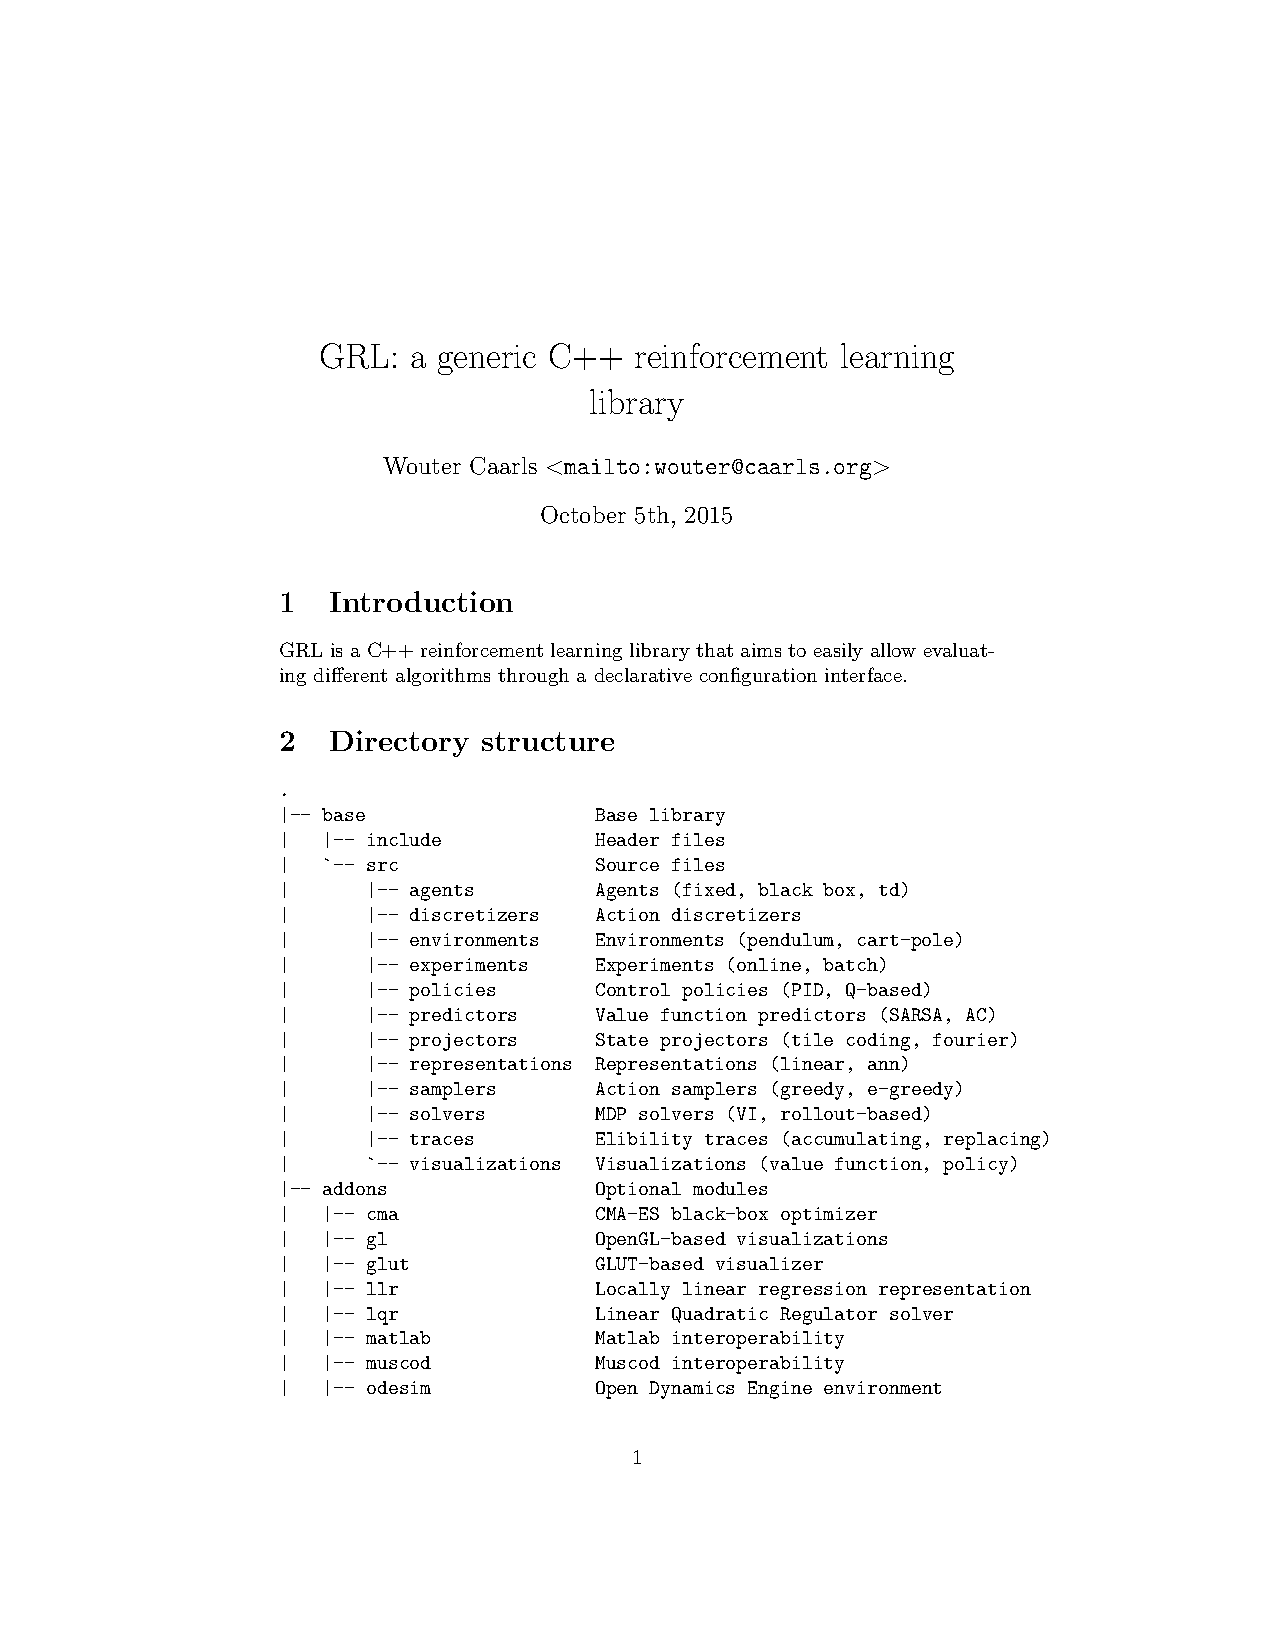
\includegraphics[width=\linewidth]{grl.png}
\caption{Python configurator user interface}
\label{fig:conf}
\end{figure}

\section{Matlab interface}

If Matlab is installed (and can be found on the path), a MEX interfaces for
the agents and environments is built. If you want to use these, make sure
that you're building with a compatible compiler, both by setting the
\txt{CC} and \txt{CXX} variables in your call to \txt{cmake} and by correctly
configuring \txt{mex}.

\subsection{Environments}

To initialize an environment, call

\begin{code}
>> spec = grl_env('cfg/matlab/pendulum_swingup.yaml');
\end{code}

Where the argument specifies a configuration file that has a top-level
'environment' tag. \txt{spec} gives some information about the environment,
such as number of dimensions, minimum and maximum values, etc. Next,
retrieve the first observation of an episode with

\begin{code}
>> o = grl_env('start');
\end{code}

where \txt{o} is the observation from the environment. All following
steps should be called using

\begin{code}
>> [o, r, t, d] = grl_env('step', a);
\end{code}

where \txt{a} is the action suggested by the agent, \txt{r} is the reward
given by the environment, \txt{t} signals termination of the episode and 
txt{d} is the length of the step.
If \txt{t} is 2, the episode ended in an absorbing state. When all episodes
are done, exit cleanly with

\begin{code}
>> grl_env('fini');
\end{code}

\subsection{Agents}

To initialize the agent, use

\begin{code}
>> grl_agent('init', 'cfg/matlab/sarsa.yaml');
\end{code}

Where the argument specifies a configuration file that has a top-level
'agent' tag. Next, give the first observation of an episode with

\begin{code}
>> a = grl_agent('start', o);
\end{code}

where \txt{o} is the observation from the environment and \txt{a} is the
action suggested by the agent. All following steps should be called using

\begin{code}
>> a = grl_agent('step', d, r, o);
\end{code}

where \txt{r} is the reward given by the environment and 
txt{d} is the length of the step. To signal the end of
an episode (absorbing state), use

\begin{code}
>> a = grl_agent('end', d, r);
\end{code}

To end an episode without an absorbing state, simply start a new one. To
exit cleanly after all epsiodes are finished (which also allows you to
reinitialize the agent with different options), call

\begin{code}
>> grl_agent('fini');
\end{code}

\appendix

\section{Agents}
\subsection{agent/black\_box}
\noindent Agent that learns from the cumulative reward of complete rollouts\\

\noindent\begin{tabular}{@{}lll@{}}
episodes&int&Number of episodes to evaluate policy\\
optimizer&optimizer&Policy optimizer\\
\end{tabular}
\subsection{agent/communicator}
\noindent Communicator agent which connects GRL to a remote agent\\

\noindent\begin{tabular}{@{}lll@{}}
communicator&communicator&Comunicator which exchanges messages with an actual/virtual environment\\
observation\_dims&int.observation\_dims&Number of observation dimensions\\
action\_dims&int.action\_dims&Number of action dimensions\\
action\_min&vector.action\_min&Lower limit of action\\
action\_max&vector.action\_max&Upper limit of action\\
test&int.test&Selection of a learning/testing agent role\\
\end{tabular}
\subsection{agent/delayed\_td}
\noindent Agent that learns from observed state transitions assuming non-integer values of control delay\\

\noindent\begin{tabular}{@{}lll@{}}
policy&mapping/policy&Control policy\\
predictor&predictor&Value function predictor\\
control\_delay&double&Relative control delay: 0 (no delay) - 1 (one timestep delay) \\
\end{tabular}
\subsection{agent/dyna}
\noindent Agent that learns from both observed and predicted state transitions\\

\noindent\begin{tabular}{@{}lll@{}}
planning\_steps&int&Number of planning steps per control step\\
planning\_horizon&int&Planning episode length\\
threads&int&Threads used for planning (0 = synchronous planning. >0 requires reentrant model\_agent)\\
policy&mapping/policy&Control policy\\
predictor&predictor&Value function predictor\\
model&observation\_model&Observation model used for planning\\
model\_predictor&predictor/model&Model predictor\\
model\_agent&agent&Agent used for planning episodes\\
\end{tabular}
\\

\noindent Provided parameters\\

\noindent\begin{tabular}{@{}lll@{}}
state&state&Current observed state of planning\\
\end{tabular}
\subsection{agent/filtering}
\noindent Agent that filters incoming observations and outgoing actions\\

\noindent\begin{tabular}{@{}lll@{}}
observation\_idx&vector&Index vector for downstream observation (-1=pad)\\
action\_idx&vector&Index vector for upstream action (-1=pad)\\
action\_dims&int&Number of downstream action dimensions\\
agent&agent&Downstream agent\\
\end{tabular}
\subsection{agent/fixed}
\noindent Fixed-policy agent\\

\noindent\begin{tabular}{@{}lll@{}}
policy&mapping/policy&Control policy\\
\end{tabular}
\subsection{agent/leo/fixed}
\noindent Leo fixed agent\\

\noindent\begin{tabular}{@{}lll@{}}
policy&mapping/policy&Control policy\\
pub\_transition\_type&signal/vector&Publisher of the transition type\\
\end{tabular}
\subsection{agent/leo/sma}
\noindent State-machine agent for Leo\\

\noindent\begin{tabular}{@{}lll@{}}
agent\_prepare&agent&Prepare agent\\
agent\_standup&agent&Safe standup agent\\
agent\_starter&agent&Starting agent\\
agent\_main&agent&Main agent\\
upright\_trigger&trigger&Trigger which finishes stand-up phase and triggers preparation agent\\
fc\_trigger&trigger&Trigger which checks for foot contact to ensure that robot is prepared to walk\\
starter\_trigger&trigger&Trigger which initiates a preprogrammed walking at the beginning\\
sub\_ic\_signal&signal/vector&Subscriber to the contact signal\\
\end{tabular}
\subsection{agent/leo/sym\_wrapper}
\noindent Leo agent that symmetrically wraps angles and controls\\

\noindent\begin{tabular}{@{}lll@{}}
agent&agent&Target agent with reduced state-action space due to symmetry\\
sub\_ic\_signal&signal/vector&Publisher of the initialization and contact signal\\
\end{tabular}
\subsection{agent/leo/td}
\noindent Leo agent that learns from observed state transitions\\

\noindent\begin{tabular}{@{}lll@{}}
policy&mapping/policy&Control policy\\
predictor&predictor&Value function predictor\\
pub\_transition\_type&signal/vector&Publisher of the transition type\\
\end{tabular}
\subsection{agent/leo\_preprogrammed}
\noindent Leo preprogrammed agent\\

\noindent\begin{tabular}{@{}lll@{}}
rand\_gen&random\_generator&Random generator for action pertubation\\
epsilon&double&Exploration rate\\
output\_min&vector.action\_min&Lower limit on outputs\\
output\_max&vector.action\_max&Upper limit on outputs\\
\end{tabular}
\subsection{agent/master/exclusive}
\noindent Master agent that selects one sub-agent to execute\\

\noindent\begin{tabular}{@{}lll@{}}
gamma&double&Discount rate\\
control\_step&double.control\_step&Characteristic step time on which gamma is defined\\
predictor&predictor&Optional (model) predictor\\
agent1&agent/sub&First subagent\\
agent2&agent/sub&Second subagent\\
\end{tabular}
\subsection{agent/master/predicated}
\noindent Master agent in which execution is predicated on preceding agent confidence\\

\noindent\begin{tabular}{@{}lll@{}}
gamma&double&Discount rate\\
control\_step&double.control\_step&Characteristic step time on which gamma is defined\\
predictor&predictor&Optional (model) predictor\\
agent1&agent/sub&First subagent\\
agent2&agent/sub&Second subagent\\
\end{tabular}
\subsection{agent/master/random}
\noindent Master agent that chooses sub-agents randomly\\

\noindent\begin{tabular}{@{}lll@{}}
gamma&double&Discount rate\\
control\_step&double.control\_step&Characteristic step time on which gamma is defined\\
predictor&predictor&Optional (model) predictor\\
agent1&agent/sub&First subagent\\
agent2&agent/sub&Second subagent\\
\end{tabular}
\subsection{agent/master/sequential}
\noindent Master agent that executes sub-agents sequentially\\

\noindent\begin{tabular}{@{}lll@{}}
predictor&predictor&Optional (model) predictor\\
agent1&agent&First subagent, providing the suggested action\\
agent2&agent&Second subagent, providing the final action\\
exporter&exporter&Optional exporter for transition log (supports time, state, observation, action, reward, terminal)\\
\end{tabular}
\subsection{agent/master/sequential/additive}
\noindent Additive master agent that executes sub-agents sequentially and adds their outputs\\

\noindent\begin{tabular}{@{}lll@{}}
predictor&predictor&Optional (model) predictor\\
agent1&agent&First subagent, providing the suggested action\\
agent2&agent&Second subagent, providing the final action\\
exporter&exporter&Optional exporter for transition log (supports time, state, observation, action, reward, terminal)\\
output\_min&vector.action\_min&Lower limit on outputs\\
output\_max&vector.action\_max&Upper limit on outputs\\
\end{tabular}
\subsection{agent/solver}
\noindent Agent that successively solves learned models of the environment\\

\noindent\begin{tabular}{@{}lll@{}}
interval&int&Episodes between successive solutions (0=asynchronous)\\
policy&mapping/policy&Control policy\\
predictor&predictor&Optional (model) predictor\\
solver&solver&Model-based solver\\
\end{tabular}
\subsection{agent/sub/compartmentalized}
\noindent Sub agent that is valid in a fixed state-space region\\

\noindent\begin{tabular}{@{}lll@{}}
min&vector.observation\_min&Minimum of compartment bounding box\\
max&vector.observation\_max&Maximum of compartment bounding box\\
agent&agent&Sub agent\\
\end{tabular}
\subsection{agent/sub/filtering}
\noindent Subagent that filters incoming observations and outgoing actions\\

\noindent\begin{tabular}{@{}lll@{}}
observation\_idx&vector&Index vector for downstream observation (-1=pad)\\
action\_idx&vector&Index vector for upstream action (-1=pad)\\
action\_dims&int&Number of downstream action dimensions\\
agent&agent/sub&Downstream subagent\\
\end{tabular}
\subsection{agent/sub/voluntary}
\noindent Sub agent that has confidence as part of the action\\

\noindent\begin{tabular}{@{}lll@{}}
dim&int&Action dimension that indicates confidence\\
agent&agent&Sub agent\\
\end{tabular}
\subsection{agent/td}
\noindent Agent that learns from observed state transitions\\

\noindent\begin{tabular}{@{}lll@{}}
policy&mapping/policy&Control policy\\
predictor&predictor&Value function predictor\\
\end{tabular}
\section{Behaviors}
\subsection{behavior/leo\_squat\_sym}
\noindent Leo squatting behavior with symmetrical switchers of observations\\

\subsection{behavior/leo\_walk}
\noindent Leo walking behavior without symmetrical switchers of observations\\

\subsection{behavior/leo\_walk\_sym}
\noindent Leo walking behavior with symmetrical switchers of observations\\

\section{Communicators}
\subsection{communicator/zeromq/pub\_sub}
\noindent Zeromq class to establish a link by sending messages asynchronously (publisher/subscriber)\\

\noindent\begin{tabular}{@{}lll@{}}
role&string&Role of the zeromq (Pub/Sub, Request/Reply)\\
sync&string&Syncronization ip address\\
pub&string&Publisher address\\
sub&string&subscriber address\\
\end{tabular}
\subsection{communicator/zeromq/request\_reply}
\noindent Zeromq class to establish a link by sending messages synchronously (request/reply)\\

\noindent\begin{tabular}{@{}lll@{}}
role&string&Role of the zeromq (Pub/Sub, Request/Reply)\\
sync&string&Syncronization ip address\\
addr&string&Address\\
\end{tabular}
\section{Converters}
\subsection{converter/state\_action\_converter}
\noindent Configurable which is capable of remapping states and actions\\

\noindent\begin{tabular}{@{}lll@{}}
state\_in&string&Comma-separated list of state elements in the input vector\\
state\_out&string&Comma-separated list of state elements in the output vector\\
action\_in&string&Comma-separated list of action elements observed in the input vector\\
action\_out&string&Comma-separated list of action elements provided in the output vector\\
\end{tabular}
\section{Discretizers}
\subsection{discretizer/peaked}
\noindent Peaked discretizer, with more resolution around center\\

\noindent\begin{tabular}{@{}lll@{}}
min&vector&Lower limit\\
max&vector&Upper limit\\
steps&vector&Discretization steps per dimension\\
peaking&vector&Extra resolution factor around center (offset by 1/factor at edges)\\
\end{tabular}
\subsection{discretizer/policy}
\noindent Returns the action suggested by a policy\\

\noindent\begin{tabular}{@{}lll@{}}
policy&mapping/policy&Policy whose action to return\\
\end{tabular}
\subsection{discretizer/split}
\noindent Compound discretizer\\

\noindent\begin{tabular}{@{}lll@{}}
identify&int&Identify active discretizer before (-1) or after (1) value\\
discretizer1&discretizer.&First discretizer\\
discretizer2&discretizer.&Second discretizer\\
\end{tabular}
\subsection{discretizer/uniform}
\noindent Uniform discretizer\\

\noindent\begin{tabular}{@{}lll@{}}
min&vector&Lower limit\\
max&vector&Upper limit\\
steps&vector&Discretization steps per dimension\\
\end{tabular}
\section{Dynamics}
\subsection{dynamics/acrobot}
\noindent Acrobot dynamics\\

\subsection{dynamics/cart\_double\_pole}
\noindent Cart-double-pole dynamics from Zhong and Rock\\

\subsection{dynamics/cart\_pole}
\noindent Cart-pole dynamics from Barto et al.\\

\subsection{dynamics/flyer2d}
\noindent 2D flyer dynamics\\

\subsection{dynamics/mountain}
\noindent Mountain world dynamics\\

\noindent\begin{tabular}{@{}lll@{}}
mass&double&Car mass\\
gravity&double&Gravitational acceleration\\
friction&double&Coefficient of viscous friction between car and ground\\
stiffness&double&Spring constant of walls\\
map&mapping/puddle&Height map\\
\end{tabular}
\subsection{dynamics/pendulum}
\noindent Pendulum dynamics based on the DCSC MOPS\\

\subsection{dynamics/rbdl}
\noindent RBDL rigid body dynamics\\

\noindent\begin{tabular}{@{}lll@{}}
file&string&RBDL Lua model file\\
options&string&Lua string to execute when loading model\\
points&string&Points\\
auxiliary&string&Model mass(mm), Center of mass (com), Center of mass velocity (comv), Angular momentum (am)\\
\end{tabular}
\subsection{dynamics/swimmer}
\noindent Coulom's swimmer dynamics\\

\noindent\begin{tabular}{@{}lll@{}}
segments&double.swimmer/segments&Number of swimmer segments\\
\end{tabular}
\subsection{dynamics/tlm}
\noindent Two-link manipulator dynamics\\

\section{Environments}
\subsection{environment/communicator}
\noindent Communicator environment which interects with a real environment by sending and receiving messages\\

\noindent\begin{tabular}{@{}lll@{}}
converter&converter&Convert states and actions if needed\\
communicator&communicator&Comunicator which exchanges messages with an actual/virtual environment\\
target\_obs\_dims&int&Observation dimension of a target\\
target\_action\_dims&int&Action dimension of a target\\
benchmark\_delays&int&Observation dimension of a target\\
\end{tabular}
\subsection{environment/leo2}
\noindent LEO/2 environment\\

\noindent\begin{tabular}{@{}lll@{}}
port&string&Device ID of FTDI usb-to-serial converter\\
bps&int&Bit rate\\
\end{tabular}
\\

\noindent Provided parameters\\

\noindent\begin{tabular}{@{}lll@{}}
state&state&Current state of the robot\\
\end{tabular}
\subsection{environment/leo\_squat}
\noindent Leo squatting environment\\

\noindent\begin{tabular}{@{}lll@{}}
behavior&behavior&Behavior type\\
xml&string&XML configuration filename\\
target\_env&environment&Interaction environment\\
observe&string&Comma-separated list of state elements observed by an agent\\
actuate&string&Comma-separated list of action elements provided by an agent\\
exporter&exporter&Optional exporter for transition log (supports time, state, observation, action, reward, terminal)\\
sub\_transition\_type&signal/vector&Subscriber to the transition type\\
pub\_ic\_signal&signal/vector&Publisher of the initialization and contact signal\\
measurement\_noise&double&Additive measurement noise\\
\end{tabular}
\\

\noindent Provided parameters\\

\noindent\begin{tabular}{@{}lll@{}}
observation\_dims&int.observation\_dims&Number of observation dimensions\\
observation\_min&vector.observation\_min&Lower limit on observations\\
observation\_max&vector.observation\_max&Upper limit on observations\\
action\_dims&int.action\_dims&Number of action dimensions\\
action\_min&vector.action\_min&Lower limit on actions\\
action\_max&vector.action\_max&Upper limit on actions\\
\end{tabular}
\subsection{environment/leo\_walk}
\noindent Leo walking environment\\

\noindent\begin{tabular}{@{}lll@{}}
behavior&behavior&Behavior type\\
xml&string&XML configuration filename\\
target\_env&environment&Interaction environment\\
observe&string&Comma-separated list of state elements observed by an agent\\
actuate&string&Comma-separated list of action elements provided by an agent\\
exporter&exporter&Optional exporter for transition log (supports time, state, observation, action, reward, terminal)\\
sub\_transition\_type&signal/vector&Subscriber to the transition type\\
pub\_ic\_signal&signal/vector&Publisher of the initialization and contact signal\\
measurement\_noise&double&Additive measurement noise\\
\end{tabular}
\\

\noindent Provided parameters\\

\noindent\begin{tabular}{@{}lll@{}}
observation\_dims&int.observation\_dims&Number of observation dimensions\\
observation\_min&vector.observation\_min&Lower limit on observations\\
observation\_max&vector.observation\_max&Upper limit on observations\\
action\_dims&int.action\_dims&Number of action dimensions\\
action\_min&vector.action\_min&Lower limit on actions\\
action\_max&vector.action\_max&Upper limit on actions\\
\end{tabular}
\subsection{environment/modeled}
\noindent Environment that uses a state transition model internally\\

\noindent\begin{tabular}{@{}lll@{}}
model&model&Environment model\\
task&task&Task to perform in the environment (should match model)\\
exporter&exporter&Optional exporter for transition log (supports time, state, observation, action, reward, terminal)\\
\end{tabular}
\\

\noindent Provided parameters\\

\noindent\begin{tabular}{@{}lll@{}}
state&signal/vector&Current state of the model\\
\end{tabular}
\subsection{environment/ode}
\noindent Open Dynamics Engine simulation environment\\

\noindent\begin{tabular}{@{}lll@{}}
xml&string&XML configuration filename\\
randomize&int&Randomize initial state\\
visualize&int&Whether to display 3D visualization\\
\end{tabular}
\\

\noindent Provided parameters\\

\noindent\begin{tabular}{@{}lll@{}}
observation\_dims&int.observation\_dims&Number of observation dimensions\\
observation\_min&vector.observation\_min&Lower limit on observations\\
observation\_max&vector.observation\_max&Upper limit on observations\\
action\_dims&int.action\_dims&Number of action dimensions\\
action\_min&vector.action\_min&Lower limit on actions\\
action\_max&vector.action\_max&Upper limit on actions\\
reward\_min&double.reward\_min&Lower limit on immediate reward\\
reward\_max&double.reward\_max&Upper limit on immediate reward\\
\end{tabular}
\subsection{environment/pre/noise}
\noindent Injects noise into an environment\\

\noindent\begin{tabular}{@{}lll@{}}
environment&environment&Environment to inject noise into\\
sensor\_noise&vector&Additive sensor noise standard deviation\\
actuator\_noise&vector&Additive actuator noise standard deviation\\
\end{tabular}
\subsection{environment/pre/shaping}
\noindent Adds reward shaping to an environment\\

\noindent\begin{tabular}{@{}lll@{}}
environment&environment&Environment to inject noise into\\
shaping\_function&mapping&Potential function over states\\
gamma&double&Discount factor\\
\end{tabular}
\subsection{environment/sandbox}
\noindent Non-Markov environment\\

\noindent\begin{tabular}{@{}lll@{}}
model&sandbox\_model&Environment model\\
task&task&Task to perform in the environment (should match model)\\
exporter&exporter&Optional exporter for transition log (supports time, state, observation, action, reward, terminal)\\
\end{tabular}
\\

\noindent Provided parameters\\

\noindent\begin{tabular}{@{}lll@{}}
state&signal/vector&Current state of the model\\
\end{tabular}
\section{Experiments}
\subsection{experiment/approx\_test}
\noindent Approximator test experiment (supervised learning)\\

\noindent\begin{tabular}{@{}lll@{}}
train\_samples&int&Number of training samples\\
test\_samples&int&Number of test samples\\
file&string&Output file (csv format)\\
input\_min&vector&Lower limit for drawing samples\\
input\_max&vector&Upper limit for drawing samples\\
projector&projector&Projector (should match representation)\\
representation&representation&Learned representation\\
mapping&mapping&Function to learn\\
\end{tabular}
\subsection{experiment/batch\_learning}
\noindent Batch learning experiment using randomly sampled experience\\

\noindent\begin{tabular}{@{}lll@{}}
runs&int&Number of separate learning runs to perform\\
batches&int&Number of batches per learning run\\
batch\_size&int&Number of transitions per batch\\
rate&int&Test trial control step frequency in Hz\\
output&string&Output base filename\\
model&model&Model in which the task is set\\
task&task&Task to be solved\\
predictor&predictor&Learner\\
test\_agent&agent&Agent to use in test trials after each batch\\
observation\_min&vector.observation\_min&Lower limit for observations\\
observation\_max&vector.observation\_max&Upper limit for observations\\
action\_min&vector.action\_min&Lower limit for actions\\
action\_max&vector.action\_max&Upper limit for actions\\
\end{tabular}
\\

\noindent Provided parameters\\

\noindent\begin{tabular}{@{}lll@{}}
state&signal/vector&Current observed state of the environment\\
\end{tabular}
\subsection{experiment/multi}
\noindent Run multiple experiments in parallel\\

\noindent\begin{tabular}{@{}lll@{}}
instances&int&Number of experiments to run in parallel\\
experiment&experiment&Experiment to run\\
\end{tabular}
\subsection{experiment/online\_learning}
\noindent Interactive learning experiment\\

\noindent\begin{tabular}{@{}lll@{}}
runs&int&Number of separate learning runs to perform\\
trials&int&Number of episodes per learning run\\
steps&int&Number of steps per learning run\\
rate&int&Control step frequency in Hz\\
test\_interval&int&Number of episodes in between test trials\\
output&string&Output base filename\\
environment&environment&Environment in which the agent acts\\
agent&agent&Agent\\
test\_agent&agent&Agent to use in test trials\\
load\_file&string&Load policy filename\\
save\_every&string&Save policy to 'output' at the end of event\\
\end{tabular}
\\

\noindent Provided parameters\\

\noindent\begin{tabular}{@{}lll@{}}
state&signal/vector&Current observed state of the environment\\
action&signal/vector&Current action applied to the environment\\
curve&signal/vector&Learning curve\\
\end{tabular}
\subsection{experiment/rpc/environment}
\noindent Environment RPC server\\

\noindent\begin{tabular}{@{}lll@{}}
port&int&Listen port\\
environment&environment&Environment to interface\\
\end{tabular}
\section{Exporters}
\subsection{exporter/csv}
\noindent Comma-separated values exporter\\

\noindent\begin{tabular}{@{}lll@{}}
file&string&Output base filename\\
fields&string&Comma-separated list of fields to write\\
style&string&Header style\\
variant&string&Variant to export\\
enabled&int&Enable writing to output file\\
\end{tabular}
\section{Importers}
\subsection{importer/csv}
\noindent Comma-separated values importer\\

\noindent\begin{tabular}{@{}lll@{}}
file&string&Input base filename\\
fields&string&Comma-separated list of fields to read\\
\end{tabular}
\section{Mappings}
\subsection{mapping/displacement}
\noindent Mapping that returns the state displacement effected by a policy\\

\noindent\begin{tabular}{@{}lll@{}}
policy&mapping/policy&Policy for which displacement is calculated\\
model&observation\_model&Observation model on which policy acts\\
\end{tabular}
\subsection{mapping/multisine}
\noindent Sum of sines mapping\\

\noindent\begin{tabular}{@{}lll@{}}
inputs&int&Number of input dimensions\\
outputs&int&Number of output dimensions\\
sines&int&Number of sines\\
\end{tabular}
\subsection{mapping/policy/action}
\noindent Policy based on a direct action representation\\

\noindent\begin{tabular}{@{}lll@{}}
sigma&vector&Standard deviation of exploration distribution\\
output\_min&vector.action\_min&Lower limit on outputs\\
output\_max&vector.action\_max&Upper limit on outputs\\
projector&projector.observation&Projects observations onto representation space\\
representation&representation.action&Action representation\\
\end{tabular}
\subsection{mapping/policy/action\_probability}
\noindent Policy based on an action-probability representation\\

\noindent\begin{tabular}{@{}lll@{}}
discretizer&discretizer&Action discretizer\\
projector&projector&Projects observation-action pairs onto representation space\\
representation&representation&Action-probability representation\\
\end{tabular}
\subsection{mapping/policy/discrete/random}
\noindent Policy that chooses discrete random actions\\

\noindent\begin{tabular}{@{}lll@{}}
discretizer&discretizer.action&Action discretizer\\
\end{tabular}
\subsection{mapping/policy/feed\_forward}
\noindent Feed-forward policy\\

\noindent\begin{tabular}{@{}lll@{}}
controls&mapping&Maps time to controls\\
\end{tabular}
\subsection{mapping/policy/mcts}
\noindent Monte-Carlo Tree Search policy\\

\noindent\begin{tabular}{@{}lll@{}}
model&observation\_model&Observation model used for planning\\
discretizer&discretizer.action&Action discretizer\\
gamma&double&Discount rate\\
epsilon&double&Exploration rate\\
horizon&int&Planning horizon\\
budget&double&Computational budget\\
\end{tabular}
\subsection{mapping/policy/parameterized/action}
\noindent Parameterized policy based on a direct action representation\\

\noindent\begin{tabular}{@{}lll@{}}
sigma&vector&Standard deviation of exploration distribution\\
output\_min&vector.action\_min&Lower limit on outputs\\
output\_max&vector.action\_max&Upper limit on outputs\\
projector&projector.observation&Projects observations onto representation space\\
representation&representation/parameterized.action&Action representation\\
\end{tabular}
\subsection{mapping/policy/parameterized/pid}
\noindent Parameterized policy based on a proportional-integral-derivative controller\\

\noindent\begin{tabular}{@{}lll@{}}
setpoint&vector&Setpoint\\
outputs&int.action\_dims&Number of outputs\\
p&vector&P gains ([out1\_in1, ..., out1\_inN, ..., outN\_in1, ..., outN\_inN])\\
i&vector&I gains\\
d&vector&D gains (use P gain on velocity instead, if available)\\
il&vector&Integration limits\\
action\_min&vector.action\_min&Lower limit on actions\\
action\_max&vector.action\_max&Upper limit on actions\\
\end{tabular}
\subsection{mapping/policy/parameterized/pidt}
\noindent Parameterized policy based on a proportional-integral-derivative controller for trajectory tracking\\

\noindent\begin{tabular}{@{}lll@{}}
trajectory&mapping&Maps time to setpoints\\
inputs&int.observation\_dims&Number of inputs\\
outputs&int.action\_dims&Number of outputs\\
p&vector&P gains ([out1\_in1, ..., out1\_inN, ..., outN\_in1, ..., outN\_inN])\\
i&vector&I gains\\
d&vector&D gains (use P gain on velocity instead, if available)\\
il&vector&Integration limits\\
action\_min&vector.action\_min&Lower limit on actions\\
action\_max&vector.action\_max&Upper limit on actions\\
\end{tabular}
\subsection{mapping/policy/parameterized/state\_feedback}
\noindent Parameterized policy based on a state feedback controller\\

\noindent\begin{tabular}{@{}lll@{}}
operating\_state&vector&Operating state around which gains are defined\\
operating\_action&vector&Operating action around which gains are defined\\
gains&vector&Gains ([in1\_out1, ..., in1\_outN, ..., inN\_out1, ..., inN\_outN])\\
output\_min&vector.action\_min&Lower action limit\\
output\_max&vector.action\_max&Upper action limit\\
\end{tabular}
\subsection{mapping/policy/post/noise}
\noindent Postprocesses policy output by injecting noise\\

\noindent\begin{tabular}{@{}lll@{}}
sigma&vector&Standard deviation of Gaussian exploration distribution\\
theta&vector&Ornstein-Uhlenbeck friction term (1=pure Gaussian noise)\\
policy&mapping/policy&Policy to inject noise into\\
\end{tabular}
\subsection{mapping/policy/random}
\noindent Policy that chooses continuous random actions\\

\noindent\begin{tabular}{@{}lll@{}}
output\_min&vector.action\_min&Lower action limit\\
output\_max&vector.action\_max&Upper action limit\\
\end{tabular}
\subsection{mapping/policy/sample\_feedback}
\noindent Policy based on state feedback controller defined over samples\\

\noindent\begin{tabular}{@{}lll@{}}
output\_min&vector.action\_min&Lower action limit\\
output\_max&vector.action\_max&Upper action limit\\
\end{tabular}
\subsection{mapping/policy/uct}
\noindent Monte-Carlo Tree Search policy using UCB1 action selection\\

\noindent\begin{tabular}{@{}lll@{}}
model&observation\_model&Observation model used for planning\\
discretizer&discretizer.action&Action discretizer\\
gamma&double&Discount rate\\
epsilon&double&Exploration rate\\
horizon&int&Planning horizon\\
budget&double&Computational budget\\
\end{tabular}
\subsection{mapping/policy/value/q}
\noindent Q-value based policy\\

\noindent\begin{tabular}{@{}lll@{}}
discretizer&discretizer.action&Action discretizer\\
projector&projector.pair&Projects observation-action pairs onto representation space\\
representation&representation.value/action&Action-value representation\\
sampler&sampler&Samples actions from action-values\\
\end{tabular}
\subsection{mapping/policy/value/q/bounded}
\noindent Q-value based policy with bounded action deltas\\

\noindent\begin{tabular}{@{}lll@{}}
bound&vector&Maximum action delta\\
discretizer&discretizer.action&Action discretizer\\
projector&projector.pair&Projects observation-action pairs onto representation space\\
representation&representation.value/action&Action-value representation\\
sampler&sampler&Samples actions from action-values\\
\end{tabular}
\subsection{mapping/policy/value/q/ucb}
\noindent UCB1 policy\\

\noindent\begin{tabular}{@{}lll@{}}
discretizer&discretizer.action&Action discretizer\\
projector&projector.pair&Projects observation-action pairs onto representation space\\
representation&representation.value/action&Q-value representation\\
visit\_representation&representation.value/action&Visit count representation\\
c\_p&double&UCB1 exploration term\\
\end{tabular}
\subsection{mapping/policy/value/v}
\noindent State-value based policy\\

\noindent\begin{tabular}{@{}lll@{}}
gamma&double&Discount rate\\
discretizer&discretizer.action&Action discretizer\\
model&observation\_model&Observation model\\
projector&projector.observation&Projects observations onto representation space\\
representation&representation.value/state&State-value representation\\
sampler&sampler&Samples actions from state-values\\
\end{tabular}
\subsection{mapping/puddle}
\noindent Random 2D puddles\\

\noindent\begin{tabular}{@{}lll@{}}
seed&int&World seed\\
smoothing&double&Standard deviation of Gaussian filter\\
steepness&double&Parameter of sigmoid stretching\\
\end{tabular}
\subsection{mapping/represented}
\noindent A mapping that internally uses a representation\\

\noindent\begin{tabular}{@{}lll@{}}
projector&projector&Projects inputs onto representation space\\
representation&representation&Representation\\
\end{tabular}
\subsection{mapping/timeline}
\noindent Imported timeline mapping\\

\noindent\begin{tabular}{@{}lll@{}}
importer&importer.dynamic&Importer with time as the first column\\
\end{tabular}
\subsection{mapping/value}
\noindent Mapping that returns the expected value of a value-based policy\\

\noindent\begin{tabular}{@{}lll@{}}
policy&mapping/policy/value&Value based policy\\
\end{tabular}
\section{Models}
\subsection{model/compass\_walker}
\noindent Simplest walker model from Garcia et al.\\

\noindent\begin{tabular}{@{}lll@{}}
control\_step&double.control\_step&Control step time\\
integration\_steps&int&Number of integration steps per control step\\
slope\_angle&double.slope\_angle&Inclination of the slope\\
\end{tabular}
\subsection{model/dynamical}
\noindent State transition model that integrates equations of motion\\

\noindent\begin{tabular}{@{}lll@{}}
control\_step&double.control\_step&Control step time\\
integration\_steps&int&Number of integration steps per control step\\
dynamics&dynamics&Equations of motion\\
\end{tabular}
\subsection{model/pinball}
\noindent Model of a ball on a plate\\

\noindent\begin{tabular}{@{}lll@{}}
control\_step&double.control\_step&Control step time\\
integration\_steps&int&Number of integration steps per control step\\
restitution&double&Coefficient of restitution\\
radius&double&Ball radius\\
maze&int&Maze ID\\
\end{tabular}
\subsection{model/puddle}
\noindent Puddle world model\\

\noindent\begin{tabular}{@{}lll@{}}
drag&double&Velocity multiplier for puddles\\
map&mapping/puddle&Puddle map\\
\end{tabular}
\subsection{model/windy}
\noindent Sutton \& Barto's windy gridworld model\\

\section{Observation\_models}
\subsection{observation\_model/approximated}
\noindent Observation model based on observed transitions\\

\noindent\begin{tabular}{@{}lll@{}}
jacobian\_step&double&Step size for Jacobian estimation\\
control\_step&double.control\_step&Control step time (0 = estimate using SMDP approximator)\\
differential&vector.differential&State dimensions for which to predict deltas\\
wrapping&vector.wrapping&Wrapping boundaries\\
observation\_min&vector.observation\_min&Lower limit on observations\\
observation\_max&vector.observation\_max&Upper limit on observations\\
stddev\_limit&double&Maximum standard deviation of acceptable predictions, as fraction of range\\
projector&projector.pair&Projector for transition model (|S|+|A| dimensions)\\
representation&representation.transition&Representation for transition model (|S|+2 dimensions)\\
\end{tabular}
\subsection{observation\_model/fixed}
\noindent Observation model based on known state transition model\\

\noindent\begin{tabular}{@{}lll@{}}
jacobian\_step&double&Step size for Jacobian estimation\\
model&model&Environment model\\
task&task&Task to perform in the environment (should match model)\\
\end{tabular}
\subsection{observation\_model/fixed\_reward}
\noindent Observation model based on observed transitions but known task\\

\noindent\begin{tabular}{@{}lll@{}}
jacobian\_step&double&Step size for Jacobian estimation\\
control\_step&double.control\_step&Control step time (0 = estimate using SMDP approximator)\\
differential&vector.differential&State dimensions for which to predict deltas\\
wrapping&vector.wrapping&Wrapping boundaries\\
observation\_min&vector.observation\_min&Lower limit on observations\\
observation\_max&vector.observation\_max&Upper limit on observations\\
stddev\_limit&double&Maximum standard deviation of acceptable predictions, as fraction of range\\
projector&projector.pair&Projector for transition model (|S|+|A| dimensions)\\
representation&representation.transition&Representation for transition model (|S|+2 dimensions)\\
task&task&Task to perform in the environment\\
\end{tabular}
\section{Optimizers}
\subsection{optimizer/cma}
\noindent Coverance matrix adaptation black-box optimizer\\

\noindent\begin{tabular}{@{}lll@{}}
population&int&Population size\\
sigma&vector&Initial standard deviation (a single-element vector will be replicated for all parameters)\\
policy&mapping/policy/parameterized&Control policy prototype\\
\end{tabular}
\subsection{optimizer/rwa}
\noindent Reward weighted averaging black-box optimizer\\

\noindent\begin{tabular}{@{}lll@{}}
mu&int&Parent population size\\
lambda&int&Offspring population size\\
sigma&vector&Standard deviation of exploration\\
policy&mapping/policy/parameterized&Control policy prototype\\
\end{tabular}
\section{Predictors}
\subsection{predictor/ac/action}
\noindent Actor-critic predictor for direct action policies\\

\noindent\begin{tabular}{@{}lll@{}}
importer&importer.static&Optional importer for pre-training\\
exporter&exporter&Optional exporter for transition log (supports observation, action, reward, next\_observation, next\_action)\\
alpha&double&Critic learning rate\\
beta&double&Actor learning rate\\
gamma&double&Discount rate\\
lambda&double&Trace decay rate\\
update\_method&string&Actor update method\\
step\_limit&vector&Actor exploration step limit\\
critic\_projector&projector.observation&Projects observations onto critic representation space\\
critic\_representation&representation.value/state&Value function representation\\
critic\_trace&trace&Trace of critic projections\\
actor\_projector&projector.observation&Projects observations onto actor representation space\\
actor\_representation&representation.action&Action representation\\
actor\_trace&trace&Trace of actor projections\\
\end{tabular}
\subsection{predictor/ac/probability}
\noindent Actor-critic predictor for action-probability policies\\

\noindent\begin{tabular}{@{}lll@{}}
importer&importer.static&Optional importer for pre-training\\
exporter&exporter&Optional exporter for transition log (supports observation, action, reward, next\_observation, next\_action)\\
alpha&double&Critic learning rate\\
beta&double&Actor learning rate\\
gamma&double&Discount rate\\
lambda&double&Trace decay rate\\
critic\_projector&projector.observation&Projects observations onto critic representation space\\
critic\_representation&representation.value/state&Value function representation\\
critic\_trace&trace&Trace of critic projections\\
actor\_projector&projector.pair&Projects observation-action pairs onto actor representation space\\
actor\_representation&representation.value/action&Action-probability representation\\
actor\_trace&trace&Trace of actor projections\\
discretizer&discretizer.action&Action discretizer\\
\end{tabular}
\subsection{predictor/ac/q}
\noindent Actor-critic predictor for direct action policies with a Q-value based critic\\

\noindent\begin{tabular}{@{}lll@{}}
importer&importer.static&Optional importer for pre-training\\
exporter&exporter&Optional exporter for transition log (supports observation, action, reward, next\_observation, next\_action)\\
alpha&double&Critic learning rate\\
beta&double&Actor learning rate\\
gamma&double&Discount rate\\
lambda&double&Trace decay rate\\
kappa&double&Advantage scaling factor\\
update\_method&string&Actor update method\\
step\_limit&vector&Actor exploration step limit\\
target&mapping&Target value at next state\\
critic\_projector&projector.pair&Projects observations onto critic representation space\\
critic\_representation&representation.value/action&Value function representation\\
critic\_trace&trace&Trace of critic projections\\
actor\_projector&projector.observation&Projects observations onto actor representation space\\
actor\_representation&representation.action&Action representation\\
actor\_trace&trace&Trace of actor projections\\
\end{tabular}
\subsection{predictor/ac/qv}
\noindent Actor-critic predictor for direct action policies with a Q critic storing advantages over a V critic\\

\noindent\begin{tabular}{@{}lll@{}}
importer&importer.static&Optional importer for pre-training\\
exporter&exporter&Optional exporter for transition log (supports observation, action, reward, next\_observation, next\_action)\\
alpha&double&Critic Q learning rate\\
beta\_v&double&Critic V learning rate\\
beta\_a&double&Actor learning rate\\
gamma&double&Discount rate\\
lambda&double&Trace decay rate\\
update\_method&string&Actor update method\\
step\_limit&vector&Actor exploration step limit\\
critic\_q\_projector&projector.pair&Projects observations onto critic Q representation space\\
critic\_q\_representation&representation.value/action&Q Value function representation\\
critic\_v\_projector&projector.observation&Projects observations onto critic V representation space\\
critic\_v\_representation&representation.value/state&V Value function representation\\
critic\_v\_trace&trace&Trace of critic V projections\\
actor\_projector&projector.observation&Projects observations onto actor representation space\\
actor\_representation&representation.action&Action representation\\
actor\_trace&trace&Trace of actor projections\\
\end{tabular}
\subsection{predictor/advantage}
\noindent Advantage learning off-policy value function predictor\\

\noindent\begin{tabular}{@{}lll@{}}
importer&importer.static&Optional importer for pre-training\\
exporter&exporter&Optional exporter for transition log (supports observation, action, reward, next\_observation, next\_action)\\
alpha&double&Learning rate\\
gamma&double&Discount rate\\
lambda&double&Trace decay rate\\
kappa&double&Advantage scaling factor\\
discretizer&discretizer.action&Action discretizer\\
projector&projector.pair&Projects observation-action pairs onto representation space\\
representation&representation.value/action&A-value representation\\
trace&trace&Trace of projections\\
\end{tabular}
\subsection{predictor/dpg}
\noindent Deterministic policy gradient predictor\\

\noindent\begin{tabular}{@{}lll@{}}
importer&importer.static&Optional importer for pre-training\\
exporter&exporter&Optional exporter for transition log (supports observation, action, reward, next\_observation, next\_action)\\
alpha&double&Advantage model learning rate\\
beta\_v&double&Critic learning rate\\
beta\_a&double&Actor learning rate\\
gamma&double&Discount rate\\
lambda&double&Trace decay rate\\
projector&projector.state&Projects observations onto representation spaces\\
critic\_representation&representation.value/state&State value function representation\\
critic\_trace&trace&Trace of critic projections\\
advantage\_representation&representation&Local advantage model representation (one output per action dimension)\\
actor\_representation&representation.action&Action representation\\
\end{tabular}
\subsection{predictor/expected\_sarsa}
\noindent Expected SARSA low-variance on-policy value function predictor\\

\noindent\begin{tabular}{@{}lll@{}}
importer&importer.static&Optional importer for pre-training\\
exporter&exporter&Optional exporter for transition log (supports observation, action, reward, next\_observation, next\_action)\\
alpha&double&Learning rate\\
gamma&double&Discount rate\\
lambda&double&Trace decay rate\\
projector&projector.pair&Projects observation-action pairs onto representation space\\
representation&representation.value/action&Q-value representation\\
policy&mapping/policy/value&Value based target policy\\
trace&trace&Trace of projections\\
\end{tabular}
\subsection{predictor/fqi}
\noindent Fitted Q-iteration predictor\\

\noindent\begin{tabular}{@{}lll@{}}
importer&importer.static&Optional importer for pre-training\\
exporter&exporter&Optional exporter for transition log (supports observation, action, reward, next\_observation, next\_action)\\
gamma&double&Discount rate\\
transitions&int&Maximum number of transitions to store\\
iterations&int&Number of policy improvement rounds per episode\\
reset\_strategy&string&At which point to reset the representation\\
macro\_batch\_size&int&Number of episodes/batches after which prediction is rebuilt. Use 0 for no rebuilds.\\
discretizer&discretizer.action&Action discretizer\\
projector&projector.pair&Projects observations onto critic representation space\\
representation&representation.value/action&Value function representation\\
\end{tabular}
\subsection{predictor/full/qi}
\noindent Deterministic model-based action-value function predictor\\

\noindent\begin{tabular}{@{}lll@{}}
importer&importer.static&Optional importer for pre-training\\
exporter&exporter&Optional exporter for transition log (supports observation, action, reward, next\_observation, next\_action)\\
gamma&double&Discount rate\\
model&observation\_model&Observation model used for planning\\
discretizer&discretizer.action&Action discretizer\\
projector&projector.pair&Projects observation-action pairs onto representation space\\
representation&representation.value/action&Action-value function representation\\
\end{tabular}
\subsection{predictor/full/vi}
\noindent Deterministic model-based state-value function predictor\\

\noindent\begin{tabular}{@{}lll@{}}
importer&importer.static&Optional importer for pre-training\\
exporter&exporter&Optional exporter for transition log (supports observation, action, reward, next\_observation, next\_action)\\
gamma&double&Discount rate\\
model&observation\_model&Observation model used for planning\\
discretizer&discretizer.action&Action discretizer\\
projector&projector.observation&Projects observations onto representation space\\
representation&representation.value/state&State-value function representation\\
\end{tabular}
\subsection{predictor/ggq}
\noindent Greedy-GQ off-policy value function predictor\\

\noindent\begin{tabular}{@{}lll@{}}
importer&importer.static&Optional importer for pre-training\\
exporter&exporter&Optional exporter for transition log (supports observation, action, reward, next\_observation, next\_action)\\
alpha&double&Learning rate\\
eta&double&Relative secondary learning rate (actual is alpha*eta)\\
gamma&double&Discount rate\\
projector&projector.pair&Projects observation-action pairs onto representation space\\
representation&representation.value/action&(Q, w) representation\\
policy&mapping/policy/value&Greedy target policy\\
\end{tabular}
\subsection{predictor/mbfqi}
\noindent Minibatch FQI predictor\\

\noindent\begin{tabular}{@{}lll@{}}
importer&importer.static&Optional importer for pre-training\\
exporter&exporter&Optional exporter for transition log (supports observation, action, reward, next\_observation, next\_action)\\
gamma&double&Discount rate\\
transitions&int&Maximum number of transitions to store\\
minibatch\_size&int&Number of transitions to average gradient over.\\
update\_interval&int&Number of minibatches between target updates.\\
discretizer&discretizer&Action discretizer\\
projector&projector.pair&Projects observations onto critic representation space\\
representation&representation.value/action&Value function representation\\
\end{tabular}
\subsection{predictor/model}
\noindent Observation model predictor\\

\noindent\begin{tabular}{@{}lll@{}}
importer&importer.static&Optional importer for pre-training\\
exporter&exporter&Optional exporter for transition log (supports observation, action, reward, next\_observation, next\_action)\\
differential&vector.differential&State dimensions for which to predict deltas\\
wrapping&vector.wrapping&Wrapping boundaries\\
projector&projector.pair&Projector for transition model (|S|+|A| dimensions)\\
representation&representation.transition&Representation for transition model (|S|+2 dimensions)\\
\end{tabular}
\subsection{predictor/multi}
\noindent Updates multiple predictors\\

\noindent\begin{tabular}{@{}lll@{}}
predictor1&predictor&First downstream predictor\\
predictor2&predictor&Second downstream predictor\\
\end{tabular}
\subsection{predictor/qv}
\noindent QV on-policy value function predictor\\

\noindent\begin{tabular}{@{}lll@{}}
importer&importer.static&Optional importer for pre-training\\
exporter&exporter&Optional exporter for transition log (supports observation, action, reward, next\_observation, next\_action)\\
alpha&double&State-action value learning rate\\
beta&double&State value learning rate\\
gamma&double&Discount rate\\
lambda&double&Trace decay rate\\
q\_projector&projector.pair&Projects observation-action pairs onto representation space\\
q\_representation&representation.value/action&State-action value representation (Q)\\
v\_projector&projector.observation&Projects observations onto representation space\\
v\_representation&representation.value/state&State value representation (V)\\
trace&trace&Trace of projections\\
\end{tabular}
\subsection{predictor/sarsa}
\noindent SARSA on-policy value function predictor\\

\noindent\begin{tabular}{@{}lll@{}}
importer&importer.static&Optional importer for pre-training\\
exporter&exporter&Optional exporter for transition log (supports observation, action, reward, next\_observation, next\_action)\\
alpha&double&Learning rate\\
gamma&double&Discount rate\\
lambda&double&Trace decay rate\\
projector&projector.pair&Projects observation-action pairs onto representation space\\
representation&representation.value/action&Q-value representation\\
trace&trace&Trace of projections\\
\end{tabular}
\subsection{predictor/td}
\noindent TD value function predictor\\

\noindent\begin{tabular}{@{}lll@{}}
importer&importer.static&Optional importer for pre-training\\
exporter&exporter&Optional exporter for transition log (supports observation, action, reward, next\_observation, next\_action)\\
alpha&double&Learning rate\\
gamma&double&Discount rate\\
lambda&double&Trace decay rate\\
projector&projector.observation&Projects observations onto representation space\\
representation&representation.value/state&State value representation\\
trace&trace&Trace of projections\\
\end{tabular}
\section{Projectors}
\subsection{projector/fourier}
\noindent Fourier basis function projector\\

\noindent\begin{tabular}{@{}lll@{}}
input\_min&vector&Lower input dimension limit (for scaling)\\
input\_max&vector&Upper input dimension limit (for scaling)\\
order&int&Order of approximation (bases per dimension)\\
parity&string&Whether to use odd or even bases\\
\end{tabular}
\\

\noindent Provided parameters\\

\noindent\begin{tabular}{@{}lll@{}}
memory&int.memory&Feature vector size\\
\end{tabular}
\subsection{projector/grid/index}
\noindent Discretizes continuous input to a linear grid index\\

\noindent\begin{tabular}{@{}lll@{}}
discretizer&discretizer&Discretizer\\
\end{tabular}
\\

\noindent Provided parameters\\

\noindent\begin{tabular}{@{}lll@{}}
memory&int.memory&Grid size\\
\end{tabular}
\subsection{projector/grid/position}
\noindent Discretizes continuous input to a grid center position\\

\noindent\begin{tabular}{@{}lll@{}}
discretizer&discretizer&Discretizer\\
\end{tabular}
\\

\noindent Provided parameters\\

\noindent\begin{tabular}{@{}lll@{}}
memory&int.memory&Grid size\\
\end{tabular}
\subsection{projector/identity}
\noindent Simply returns the input vector\\

\subsection{projector/monomial}
\noindent Monomial basis function projector\\

\noindent\begin{tabular}{@{}lll@{}}
operating\_input&vector&Origin\\
degree&int&Maximum degree of monomials\\
\end{tabular}
\\

\noindent Provided parameters\\

\noindent\begin{tabular}{@{}lll@{}}
memory&int.memory&Feature vector size\\
\end{tabular}
\subsection{projector/multi}
\noindent Combines multiple projections\\

\noindent\begin{tabular}{@{}lll@{}}
dim&int&Indicator dimension (-1=union)\\
projector1&projector.&First downstream projector\\
projector2&projector.&Second downstream projector\\
memories&vector.memory&Memory of downstream projectors\\
\end{tabular}
\\

\noindent Provided parameters\\

\noindent\begin{tabular}{@{}lll@{}}
memory&int.memory&Feature vector size\\
\end{tabular}
\subsection{projector/pre/normalizing}
\noindent Preprocesses projection onto a normalized [0, 1] vector\\

\noindent\begin{tabular}{@{}lll@{}}
input\_min&vector&Lower input dimension limit (for scaling)\\
input\_max&vector&Upper input dimension limit (for scaling)\\
projector&projector.&Downstream projector\\
\end{tabular}
\subsection{projector/pre/peaked}
\noindent Preprocesses projection for more resolution around center\\

\noindent\begin{tabular}{@{}lll@{}}
peaking&vector&Extra resolution factor around center (offset by 1/factor at edges)\\
input\_min&vector&Lower input dimension limit (for scaling)\\
input\_max&vector&Upper input dimension limit (for scaling)\\
projector&projector.&Downstream projector\\
\end{tabular}
\subsection{projector/pre/scaling}
\noindent Preprocesses projection onto a scaled vector\\

\noindent\begin{tabular}{@{}lll@{}}
scaling&vector&Scaling vector\\
projector&projector.&Downstream projector\\
\end{tabular}
\subsection{projector/rbf}
\noindent Projection on a grid of triangular radial basis functions\\

\noindent\begin{tabular}{@{}lll@{}}
input\_min&vector&Lower input dimension limit\\
input\_max&vector&Upper input dimension limit\\
steps&vector&Basis functions per dimension\\
\end{tabular}
\\

\noindent Provided parameters\\

\noindent\begin{tabular}{@{}lll@{}}
memory&int.memory&RBF size\\
\end{tabular}
\subsection{projector/sample/ann}
\noindent Projects onto samples found through approximate nearest-neighbor search\\

\noindent\begin{tabular}{@{}lll@{}}
samples&int&Maximum number of samples to store\\
neighbors&int&Number of neighbors to return\\
locality&double&Locality of weighing function\\
interval&int&Samples to accumulate before rebuilding kd-tree\\
incremental&int&Search samples that haven't been indexed yet\\
bucket\_size&int&?\\
error\_bound&double&?\\
inputs&int&Number of input dimensions\\
\end{tabular}
\subsection{projector/sample/ertree}
\noindent Projects onto samples found through the Extra-trees algorithm by Geurts et al.\\

\noindent\begin{tabular}{@{}lll@{}}
samples&int&Maximum number of samples to store\\
trees&int&Number of trees in the forest\\
splits&int&Number of candidate splits\\
leaf\_size&int&Maximum number of samples in a leaf\\
inputs&int&Number of input dimensions\\
outputs&int&Number of output dimensions\\
\end{tabular}
\subsection{projector/split}
\noindent Splits a feature vector into distinct sets\\

\noindent\begin{tabular}{@{}lll@{}}
index&vector&Binary vector that specifies which dimensions to use as index\\
discretizer&discretizer&Determines the distinct set based on the index dimensions\\
projector&projector&Projects the non-index dimensions onto a feature vector\\
projector\_memory&int.memory&Memory of downstream projector\\
\end{tabular}
\\

\noindent Provided parameters\\

\noindent\begin{tabular}{@{}lll@{}}
memory&int.memory&Resulting feature vector size\\
\end{tabular}
\subsection{projector/tile\_coding}
\noindent Hashed tile coding projector\\

\noindent\begin{tabular}{@{}lll@{}}
tilings&int&Number of tilings\\
memory&int.memory&Hash table size\\
safe&int&Collision detection (0=off, 1=claim on write, 2=claim always)\\
resolution&vector&Size of a single tile\\
wrapping&vector.wrapping&Wrapping boundaries (must be multiple of resolution)\\
\end{tabular}
\section{Random\_generators}
\subsection{random\_generator/normal}
\noindent Normal Random generator\\

\noindent\begin{tabular}{@{}lll@{}}
mu&double&Mean\\
sigma&double&Standart deviation\\
\end{tabular}
\subsection{random\_generator/ornstein\_uhlenbeck}
\noindent Ornstein-Uhlenbeck Random generator\\

\noindent\begin{tabular}{@{}lll@{}}
center&double&Attraction point\\
theta&double&Theta\\
sigma&double&Sigma\\
\end{tabular}
\subsection{random\_generator/uniform}
\noindent Uniform Random generator\\

\noindent\begin{tabular}{@{}lll@{}}
lower&double&Lower bound of an interval\\
upper&double&Upper bound of an interval\\
\end{tabular}
\subsection{random\_generator/uniform\_integer}
\noindent Uniform Integer Random generator\\

\noindent\begin{tabular}{@{}lll@{}}
ma&int&Upper bound of an interval [0, ma)\\
\end{tabular}
\section{Representations}
\subsection{representation/additive}
\noindent Linear combination of two representations\\

\noindent\begin{tabular}{@{}lll@{}}
representation1&representation.&First representation\\
representation2&representation.&Second representation\\
learning&int&Which representation to learn (0=both)\\
\end{tabular}
\subsection{representation/communicator}
\noindent Interface to an out-of-process representation\\

\noindent\begin{tabular}{@{}lll@{}}
inputs&int&Number of input dimensions\\
outputs&int&Number of output dimensions\\
communicator&communicator&Communicator which exchanges messages with the out-of-process representation\\
\end{tabular}
\subsection{representation/dictionary}
\noindent Stores examples as key-value pairs in a dictionary\\

\subsection{representation/iterative}
\noindent Representation that iteratively trains a sub-representation\\

\noindent\begin{tabular}{@{}lll@{}}
epochs&int&Learning epochs\\
cumulative&int&Add to training set instead of replacing it\\
representation&representation.&Downstream representation\\
\end{tabular}
\subsection{representation/llr}
\noindent Performs locally linear regression through samples\\

\noindent\begin{tabular}{@{}lll@{}}
ridge&double&Ridge regression (Tikhonov) factor\\
order&int&Order of regression model\\
input\_nominals&vector&Vector indicating which input dimensions are nominal\\
output\_nominals&vector&Vector indicating which output dimensions are nominal\\
outputs&int&Number of output dimensions\\
output\_min&vector&Lower output limit\\
output\_max&vector&Upper output limit\\
projector&projector/sample&Projector used to generate input for this representation\\
\end{tabular}
\subsection{representation/parameterized/ann}
\noindent Parameterized artificial neural network representation\\

\noindent\begin{tabular}{@{}lll@{}}
inputs&int&Number of input dimensions\\
outputs&int&Number of output dimensions\\
hiddens&vector&Number of hidden nodes per layer\\
eta&double&Learning rate (0=RPROP, <0=RMSPROP)\\
\end{tabular}
\subsection{representation/parameterized/linear}
\noindent Linear-in-parameters representation\\

\noindent\begin{tabular}{@{}lll@{}}
init\_min&vector&Lower initial value limit\\
init\_max&vector&Upper initial value limit\\
memory&int.memory&Feature vector size\\
outputs&int&Number of outputs\\
output\_min&vector&Lower output limit\\
output\_max&vector&Upper output limit\\
\end{tabular}
\section{Samplers}
\subsection{sampler/ac\_ornstein\_ohlenbeck}
\noindent Action-correlated maximum search with an Ornstein-Uhlenbeck random chance of non-maximums\\

\noindent\begin{tabular}{@{}lll@{}}
rand\_max&int&In case of multiple maximumum values select a random index among them\\
discretizer&discretizer.action&Action discretizer\\
theta&vector&Theta parameter of Ornstein-Uhlenbeck\\
sigma&vector&Sigma parameter of Ornstein-Uhlenbeck\\
center&vector&Centering parameter of Ornstein-Uhlenbeck\\
pub\_sub\_ou\_state&signal/vector&Publisher and subscriber to the value of noise (or action in the ACOU case) of the Ornstein Uhlenbeck familiy of samplers\\
epsilon&double&Exploration rate\\
\end{tabular}
\subsection{sampler/epsilon\_greedy}
\noindent Maximum search with a uniform random chance of non-maximums\\

\noindent\begin{tabular}{@{}lll@{}}
rand\_max&int&In case of multiple maximumum values select a random index among them\\
epsilon&vector&Exploration rate (can be defined per action)\\
\end{tabular}
\subsection{sampler/epsilon\_ornstein\_ohlenbeck}
\noindent Exploitations are done by greedy action selection without constraints, as in e-greedy. Explorations are done with time-correlated noise, as it is in OU.\\

\noindent\begin{tabular}{@{}lll@{}}
rand\_max&int&In case of multiple maximumum values select a random index among them\\
discretizer&discretizer.action&Action discretizer\\
theta&vector&Theta parameter of Ornstein-Uhlenbeck\\
sigma&vector&Sigma parameter of Ornstein-Uhlenbeck\\
center&vector&Centering parameter of Ornstein-Uhlenbeck\\
pub\_sub\_ou\_state&signal/vector&Publisher and subscriber to the value of noise (or action in the ACOU case) of the Ornstein Uhlenbeck familiy of samplers\\
epsilon&double&Exploration rate\\
\end{tabular}
\subsection{sampler/epsilon\_pada}
\noindent exploitations are done by greedy action selection without constraints, as in e-greedy. Explorations are done with constrained set of actions, as it is in pada.\\

\noindent\begin{tabular}{@{}lll@{}}
rand\_max&int&In case of multiple maximumum values select a random index among them\\
epsilon&vector&Exploration rate (can be defined per action)\\
discretizer&discretizer.action&Action discretizer\\
delta&vector&Delta of PADA\\
pub\_sub\_pada\_state&signal/vector&Publisher and subscriber to the value of action of the PADA familiy of samplers\\
\end{tabular}
\subsection{sampler/greedy}
\noindent Maximum search\\

\noindent\begin{tabular}{@{}lll@{}}
rand\_max&int&In case of multiple maximumum values select a random index among them\\
\end{tabular}
\subsection{sampler/leo/action}
\noindent Wrapper for an action sampler for Leo (can modify memory of samplers with memory at contact events)\\

\noindent\begin{tabular}{@{}lll@{}}
sampler&sampler&Samples actions from action-values\\
sub\_ic\_signal&signal/vector&Subscrider to the initialization and contact signal\\
pub\_sub\_sampler\_state&signal/vector&Publisher and subscriber of the sampler state with memory such as previous action, noise, etc.\\
\end{tabular}
\subsection{sampler/ornstein\_ohlenbeck}
\noindent Maximum search with an Ornstein-Uhlenbeck random chance of non-maximums\\

\noindent\begin{tabular}{@{}lll@{}}
rand\_max&int&In case of multiple maximumum values select a random index among them\\
discretizer&discretizer.action&Action discretizer\\
theta&vector&Theta parameter of Ornstein-Uhlenbeck\\
sigma&vector&Sigma parameter of Ornstein-Uhlenbeck\\
center&vector&Centering parameter of Ornstein-Uhlenbeck\\
pub\_sub\_ou\_state&signal/vector&Publisher and subscriber to the value of noise (or action in the ACOU case) of the Ornstein Uhlenbeck familiy of samplers\\
\end{tabular}
\subsection{sampler/pada}
\noindent Maximum search with a PADA random chance of non-maximums\\

\noindent\begin{tabular}{@{}lll@{}}
rand\_max&int&In case of multiple maximumum values select a random index among them\\
epsilon&vector&Exploration rate (can be defined per action)\\
discretizer&discretizer.action&Action discretizer\\
delta&vector&Delta of PADA\\
pub\_sub\_pada\_state&signal/vector&Publisher and subscriber to the value of action of the PADA familiy of samplers\\
\end{tabular}
\subsection{sampler/pada\_ornstein\_ohlenbeck}
\noindent Explorations and exploitations are same as OU, but action is selected from a constrained set, as in PADA. \\

\noindent\begin{tabular}{@{}lll@{}}
rand\_max&int&In case of multiple maximumum values select a random index among them\\
discretizer&discretizer.action&Action discretizer\\
theta&vector&Theta parameter of Ornstein-Uhlenbeck\\
sigma&vector&Sigma parameter of Ornstein-Uhlenbeck\\
center&vector&Centering parameter of Ornstein-Uhlenbeck\\
pub\_sub\_ou\_state&signal/vector&Publisher and subscriber to the value of noise (or action in the ACOU case) of the Ornstein Uhlenbeck familiy of samplers\\
pada&sampler&Pada sampler\\
pub\_new\_action&signal/vector&Publisher of the signal with noise\\
\end{tabular}
\subsection{sampler/softmax}
\noindent Softmax (Gibbs/Boltzmann) sampler\\

\noindent\begin{tabular}{@{}lll@{}}
tau&double&Temperature of Boltzmann distribution\\
\end{tabular}
\section{Sandbox\_models}
\subsection{sandbox\_model/compass\_walker}
\noindent Simplest walker model from Garcia et al. with a sequential evaluation\\

\noindent\begin{tabular}{@{}lll@{}}
control\_step&double.control\_step&Control step time\\
integration\_steps&int&Number of integration steps per control step\\
slope\_angle&double.slope\_angle&Inclination of the slope\\
exporter&exporter&Optional exporter for transition log (supports time, state, observation, action, reward, terminal)\\
use\_avg\_velocity&int&Velocity type \\
\end{tabular}
\subsection{sandbox\_model/leo\_squatting}
\noindent State transition model that integrates equations of motion and augments state vector with additional elements\\

\noindent\begin{tabular}{@{}lll@{}}
control\_step&double.control\_step&Control step time\\
integration\_steps&int&Number of integration steps per control step\\
dynamics&dynamics/rbdl&Equations of motion\\
target\_dof&int.target\_dof&Number of degrees of freedom of the target model\\
animation&string&Save current state or full animation\\
target\_env&environment&Interaction environment\\
lower\_height&double.lower\_height&Lower bound of root height to switch direction\\
upper\_height&double.upper\_height&Upper bound of root height to switch direction\\
\end{tabular}
\section{Signals}
\subsection{signal/matrix}
\noindent Matrix-based signal (trajectory, etc.)\\

\subsection{signal/vector}
\noindent Vector-based signal (state, observation, etc.)\\

\section{Solvers}
\subsection{solver/agent}
\noindent Solver that uses a simulated agent\\

\noindent\begin{tabular}{@{}lll@{}}
steps&int&Number of planning steps before solution is returned\\
horizon&int&Planning episode length\\
start&vector&Starting state for planning\\
model&observation\_model&Observation model used for planning\\
agent&agent&Agent used for planning episodes\\
\end{tabular}
\\

\noindent Provided parameters\\

\noindent\begin{tabular}{@{}lll@{}}
state&state&Current observed state of planning\\
\end{tabular}
\subsection{solver/ilqg}
\noindent Iterative Linear Quadratic Gaussian trajectory optimizer\\

\noindent\begin{tabular}{@{}lll@{}}
horizon&int&Horizon\\
iterations&int&Maximum number of iterations\\
stddev&vector&Standard deviation of initial random action sequence\\
regularization&string&Regularization method\\
model&observation\_model&Observation model\\
policy&mapping/policy/sample\_feedback&Sample feedback policy to adjust\\
\end{tabular}
\\

\noindent Provided parameters\\

\noindent\begin{tabular}{@{}lll@{}}
trajectory&signal/matrix&Predicted trajectory\\
\end{tabular}
\subsection{solver/lqr}
\noindent Linear Quadratic Regulator solver\\

\noindent\begin{tabular}{@{}lll@{}}
operating\_state&vector&Operating state around which to linearize\\
operating\_action&vector&Operating action around which to linearize\\
model&observation\_model&Observation model\\
policy&mapping/policy/parameterized/state\_feedback&State feedback policy to adjust\\
\end{tabular}
\subsection{solver/vi}
\noindent Value iteration solver\\

\noindent\begin{tabular}{@{}lll@{}}
sweeps&int&Number of planning sweeps before solution is returned\\
parallel&int&Perform backups in parallel (requires reentrant representation)\\
discretizer&discretizer.observation&State space discretizer\\
predictor&predictor/full&Predictor to iterate\\
\end{tabular}
\section{Tasks}
\subsection{task/acrobot/balancing}
\noindent Acrobot balancing task\\

\noindent Provided parameters\\

\noindent\begin{tabular}{@{}lll@{}}
observation\_dims&int.observation\_dims&Number of observation dimensions\\
observation\_min&vector.observation\_min&Lower limit on observations\\
observation\_max&vector.observation\_max&Upper limit on observations\\
action\_dims&int.action\_dims&Number of action dimensions\\
action\_min&vector.action\_min&Lower limit on actions\\
action\_max&vector.action\_max&Upper limit on actions\\
reward\_min&double.reward\_min&Lower limit on immediate reward\\
reward\_max&double.reward\_max&Upper limit on immediate reward\\
\end{tabular}
\subsection{task/acrobot/regulator}
\noindent Acrobot regulator task\\

\noindent\begin{tabular}{@{}lll@{}}
start&vector&Starting state\\
goal&vector&Goal state\\
stddev&vector&Starting state standard deviation\\
q&vector&Q (state cost) matrix diagonal\\
r&vector&R (action cost) matrix diagonal\\
function&string&Cost function style\\
smoothing&double&Cost function smoothing parameter\\
\end{tabular}
\\

\noindent Provided parameters\\

\noindent\begin{tabular}{@{}lll@{}}
observation\_dims&int.observation\_dims&Number of observation dimensions\\
observation\_min&vector.observation\_min&Lower limit on observations\\
observation\_max&vector.observation\_max&Upper limit on observations\\
action\_dims&int.action\_dims&Number of action dimensions\\
action\_min&vector.action\_min&Lower limit on actions\\
action\_max&vector.action\_max&Upper limit on actions\\
reward\_min&double.reward\_min&Lower limit on immediate reward\\
reward\_max&double.reward\_max&Upper limit on immediate reward\\
\end{tabular}
\subsection{task/cart\_double\_pole/balancing}
\noindent Cart-double-pole balancing task\\

\noindent\begin{tabular}{@{}lll@{}}
timeout&double&Episode timeout\\
\end{tabular}
\\

\noindent Provided parameters\\

\noindent\begin{tabular}{@{}lll@{}}
observation\_dims&int.observation\_dims&Number of observation dimensions\\
observation\_min&vector.observation\_min&Lower limit on observations\\
observation\_max&vector.observation\_max&Upper limit on observations\\
action\_dims&int.action\_dims&Number of action dimensions\\
action\_min&vector.action\_min&Lower limit on actions\\
action\_max&vector.action\_max&Upper limit on actions\\
reward\_min&double.reward\_min&Lower limit on immediate reward\\
reward\_max&double.reward\_max&Upper limit on immediate reward\\
\end{tabular}
\subsection{task/cart\_double\_pole/regulator}
\noindent Cart-double-pole regulator task\\

\noindent\begin{tabular}{@{}lll@{}}
start&vector&Starting state\\
goal&vector&Goal state\\
stddev&vector&Starting state standard deviation\\
q&vector&Q (state cost) matrix diagonal\\
r&vector&R (action cost) matrix diagonal\\
function&string&Cost function style\\
smoothing&double&Cost function smoothing parameter\\
timeout&double&Episode timeout\\
\end{tabular}
\\

\noindent Provided parameters\\

\noindent\begin{tabular}{@{}lll@{}}
observation\_dims&int.observation\_dims&Number of observation dimensions\\
observation\_min&vector.observation\_min&Lower limit on observations\\
observation\_max&vector.observation\_max&Upper limit on observations\\
action\_dims&int.action\_dims&Number of action dimensions\\
action\_min&vector.action\_min&Lower limit on actions\\
action\_max&vector.action\_max&Upper limit on actions\\
reward\_min&double.reward\_min&Lower limit on immediate reward\\
reward\_max&double.reward\_max&Upper limit on immediate reward\\
\end{tabular}
\subsection{task/cart\_double\_pole/swingup}
\noindent Cart-double-pole swing-up task\\

\noindent\begin{tabular}{@{}lll@{}}
timeout&double&Episode timeout\\
\end{tabular}
\\

\noindent Provided parameters\\

\noindent\begin{tabular}{@{}lll@{}}
observation\_dims&int.observation\_dims&Number of observation dimensions\\
observation\_min&vector.observation\_min&Lower limit on observations\\
observation\_max&vector.observation\_max&Upper limit on observations\\
action\_dims&int.action\_dims&Number of action dimensions\\
action\_min&vector.action\_min&Lower limit on actions\\
action\_max&vector.action\_max&Upper limit on actions\\
reward\_min&double.reward\_min&Lower limit on immediate reward\\
reward\_max&double.reward\_max&Upper limit on immediate reward\\
\end{tabular}
\subsection{task/cart\_pole/balancing}
\noindent Cart-pole balancing task\\

\noindent\begin{tabular}{@{}lll@{}}
timeout&double&Episode timeout\\
\end{tabular}
\\

\noindent Provided parameters\\

\noindent\begin{tabular}{@{}lll@{}}
observation\_dims&int.observation\_dims&Number of observation dimensions\\
observation\_min&vector.observation\_min&Lower limit on observations\\
observation\_max&vector.observation\_max&Upper limit on observations\\
action\_dims&int.action\_dims&Number of action dimensions\\
action\_min&vector.action\_min&Lower limit on actions\\
action\_max&vector.action\_max&Upper limit on actions\\
reward\_min&double.reward\_min&Lower limit on immediate reward\\
reward\_max&double.reward\_max&Upper limit on immediate reward\\
\end{tabular}
\subsection{task/cart\_pole/regulator}
\noindent Cart-pole regulator task\\

\noindent\begin{tabular}{@{}lll@{}}
start&vector&Starting state\\
goal&vector&Goal state\\
stddev&vector&Starting state standard deviation\\
q&vector&Q (state cost) matrix diagonal\\
r&vector&R (action cost) matrix diagonal\\
function&string&Cost function style\\
smoothing&double&Cost function smoothing parameter\\
timeout&double&Episode timeout\\
\end{tabular}
\\

\noindent Provided parameters\\

\noindent\begin{tabular}{@{}lll@{}}
observation\_dims&int.observation\_dims&Number of observation dimensions\\
observation\_min&vector.observation\_min&Lower limit on observations\\
observation\_max&vector.observation\_max&Upper limit on observations\\
action\_dims&int.action\_dims&Number of action dimensions\\
action\_min&vector.action\_min&Lower limit on actions\\
action\_max&vector.action\_max&Upper limit on actions\\
reward\_min&double.reward\_min&Lower limit on immediate reward\\
reward\_max&double.reward\_max&Upper limit on immediate reward\\
\end{tabular}
\subsection{task/cart\_pole/swingup}
\noindent Cart-pole swing-up task\\

\noindent\begin{tabular}{@{}lll@{}}
timeout&double&Episode timeout\\
randomization&int&Start state randomization\\
shaping&int&Whether to use reward shaping\\
gamma&double&Discount rate for reward shaping\\
end\_stop\_penalty&int&Terminate episode with penalty when end stop is reached\\
\end{tabular}
\\

\noindent Provided parameters\\

\noindent\begin{tabular}{@{}lll@{}}
observation\_dims&int.observation\_dims&Number of observation dimensions\\
observation\_min&vector.observation\_min&Lower limit on observations\\
observation\_max&vector.observation\_max&Upper limit on observations\\
action\_dims&int.action\_dims&Number of action dimensions\\
action\_min&vector.action\_min&Lower limit on actions\\
action\_max&vector.action\_max&Upper limit on actions\\
reward\_min&double.reward\_min&Lower limit on immediate reward\\
reward\_max&double.reward\_max&Upper limit on immediate reward\\
\end{tabular}
\subsection{task/compass\_walker/vref}
\noindent Compass walker tracking velocity task\\

\noindent\begin{tabular}{@{}lll@{}}
timeout&double&Learning episode timeout\\
initial\_state\_variation&double&Variation of initial state\\
slope\_angle&double.slope\_angle&Inclination of the slope\\
negative\_reward&double&Negative reward\\
observe&vector&State elements observed by an agent\\
steps&int&number of steps after which task is terminated\\
reference\_velocity&double&Reference velocity\\
per\_step\_reward&int&If set, give reward per every step\\
\end{tabular}
\\

\noindent Provided parameters\\

\noindent\begin{tabular}{@{}lll@{}}
observation\_dims&int.observation\_dims&Number of observation dimensions\\
observation\_min&vector.observation\_min&Lower limit on observations\\
observation\_max&vector.observation\_max&Upper limit on observations\\
action\_dims&int.action\_dims&Number of action dimensions\\
action\_min&vector.action\_min&Lower limit on actions\\
action\_max&vector.action\_max&Upper limit on actions\\
reward\_min&double.reward\_min&Lower limit on immediate reward\\
reward\_max&double.reward\_max&Upper limit on immediate reward\\
\end{tabular}
\subsection{task/compass\_walker/vrefu}
\noindent Compass walker tracking velocity task with controls minimization\\

\noindent\begin{tabular}{@{}lll@{}}
timeout&double&Learning episode timeout\\
initial\_state\_variation&double&Variation of initial state\\
slope\_angle&double.slope\_angle&Inclination of the slope\\
negative\_reward&double&Negative reward\\
observe&vector&State elements observed by an agent\\
steps&int&number of steps after which task is terminated\\
reference\_velocity&double&Reference velocity\\
per\_step\_reward&int&If set, give reward per every step\\
\end{tabular}
\\

\noindent Provided parameters\\

\noindent\begin{tabular}{@{}lll@{}}
observation\_dims&int.observation\_dims&Number of observation dimensions\\
observation\_min&vector.observation\_min&Lower limit on observations\\
observation\_max&vector.observation\_max&Upper limit on observations\\
action\_dims&int.action\_dims&Number of action dimensions\\
action\_min&vector.action\_min&Lower limit on actions\\
action\_max&vector.action\_max&Upper limit on actions\\
reward\_min&double.reward\_min&Lower limit on immediate reward\\
reward\_max&double.reward\_max&Upper limit on immediate reward\\
\end{tabular}
\subsection{task/compass\_walker/walk}
\noindent Compass walker walking task\\

\noindent\begin{tabular}{@{}lll@{}}
timeout&double&Learning episode timeout\\
initial\_state\_variation&double&Variation of initial state\\
slope\_angle&double.slope\_angle&Inclination of the slope\\
negative\_reward&double&Negative reward\\
observe&vector&State elements observed by an agent\\
steps&int&number of steps after which task is terminated\\
\end{tabular}
\\

\noindent Provided parameters\\

\noindent\begin{tabular}{@{}lll@{}}
observation\_dims&int.observation\_dims&Number of observation dimensions\\
observation\_min&vector.observation\_min&Lower limit on observations\\
observation\_max&vector.observation\_max&Upper limit on observations\\
action\_dims&int.action\_dims&Number of action dimensions\\
action\_min&vector.action\_min&Lower limit on actions\\
action\_max&vector.action\_max&Upper limit on actions\\
reward\_min&double.reward\_min&Lower limit on immediate reward\\
reward\_max&double.reward\_max&Upper limit on immediate reward\\
\end{tabular}
\subsection{task/flyer2d/regulator}
\noindent 2D flyer regulator task\\

\noindent\begin{tabular}{@{}lll@{}}
start&vector&Starting state\\
goal&vector&Goal state\\
stddev&vector&Starting state standard deviation\\
q&vector&Q (state cost) matrix diagonal\\
r&vector&R (action cost) matrix diagonal\\
function&string&Cost function style\\
smoothing&double&Cost function smoothing parameter\\
action\_range&double&Range of allowed actions\\
timeout&double&Episode timeout\\
\end{tabular}
\\

\noindent Provided parameters\\

\noindent\begin{tabular}{@{}lll@{}}
observation\_dims&int.observation\_dims&Number of observation dimensions\\
observation\_min&vector.observation\_min&Lower limit on observations\\
observation\_max&vector.observation\_max&Upper limit on observations\\
action\_dims&int.action\_dims&Number of action dimensions\\
action\_min&vector.action\_min&Lower limit on actions\\
action\_max&vector.action\_max&Upper limit on actions\\
reward\_min&double.reward\_min&Lower limit on immediate reward\\
reward\_max&double.reward\_max&Upper limit on immediate reward\\
\end{tabular}
\subsection{task/leo\_squatting}
\noindent Task specification for Leo squatting with a fixed arm\\

\noindent\begin{tabular}{@{}lll@{}}
timeout&double.timeout&Task timeout\\
rand\_init&int.rand\_init&Initialization from a random pose\\
\end{tabular}
\\

\noindent Provided parameters\\

\noindent\begin{tabular}{@{}lll@{}}
observation\_dims&int.observation\_dims&Number of observation dimensions\\
observation\_min&vector.observation\_min&Lower limit on observations\\
observation\_max&vector.observation\_max&Upper limit on observations\\
action\_dims&int.action\_dims&Number of action dimensions\\
action\_min&vector.action\_min&Lower limit on actions\\
action\_max&vector.action\_max&Upper limit on actions\\
reward\_min&double.reward\_min&Lower limit on immediate reward\\
reward\_max&double.reward\_max&Upper limit on immediate reward\\
\end{tabular}
\subsection{task/lua}
\noindent User-provided task specification in LUA\\

\noindent\begin{tabular}{@{}lll@{}}
file&string&Lua task file\\
options&string&Lua string to execute when loading task\\
\end{tabular}
\\

\noindent Provided parameters\\

\noindent\begin{tabular}{@{}lll@{}}
observation\_dims&int.observation\_dims&Number of observation dimensions\\
observation\_min&vector.observation\_min&Lower limit on observations\\
observation\_max&vector.observation\_max&Upper limit on observations\\
action\_dims&int.action\_dims&Number of action dimensions\\
action\_min&vector.action\_min&Lower limit on actions\\
action\_max&vector.action\_max&Upper limit on actions\\
reward\_min&double.reward\_min&Lower limit on immediate reward\\
reward\_max&double.reward\_max&Upper limit on immediate reward\\
\end{tabular}
\subsection{task/mountain/regulator}
\noindent Mountain world regulator task\\

\noindent\begin{tabular}{@{}lll@{}}
start&vector&Starting state\\
goal&vector&Goal state\\
stddev&vector&Starting state standard deviation\\
q&vector&Q (state cost) matrix diagonal\\
r&vector&R (action cost) matrix diagonal\\
function&string&Cost function style\\
smoothing&double&Cost function smoothing parameter\\
\end{tabular}
\\

\noindent Provided parameters\\

\noindent\begin{tabular}{@{}lll@{}}
observation\_dims&int.observation\_dims&Number of observation dimensions\\
observation\_min&vector.observation\_min&Lower limit on observations\\
observation\_max&vector.observation\_max&Upper limit on observations\\
action\_dims&int.action\_dims&Number of action dimensions\\
action\_min&vector.action\_min&Lower limit on actions\\
action\_max&vector.action\_max&Upper limit on actions\\
reward\_min&double.reward\_min&Lower limit on immediate reward\\
reward\_max&double.reward\_max&Upper limit on immediate reward\\
\end{tabular}
\subsection{task/pendulum/regulator}
\noindent Pendulum regulator task\\

\noindent\begin{tabular}{@{}lll@{}}
start&vector&Starting state\\
goal&vector&Goal state\\
stddev&vector&Starting state standard deviation\\
q&vector&Q (state cost) matrix diagonal\\
r&vector&R (action cost) matrix diagonal\\
function&string&Cost function style\\
smoothing&double&Cost function smoothing parameter\\
\end{tabular}
\\

\noindent Provided parameters\\

\noindent\begin{tabular}{@{}lll@{}}
observation\_dims&int.observation\_dims&Number of observation dimensions\\
observation\_min&vector.observation\_min&Lower limit on observations\\
observation\_max&vector.observation\_max&Upper limit on observations\\
action\_dims&int.action\_dims&Number of action dimensions\\
action\_min&vector.action\_min&Lower limit on actions\\
action\_max&vector.action\_max&Upper limit on actions\\
reward\_min&double.reward\_min&Lower limit on immediate reward\\
reward\_max&double.reward\_max&Upper limit on immediate reward\\
\end{tabular}
\subsection{task/pendulum/swingup}
\noindent Pendulum swing-up task\\

\noindent\begin{tabular}{@{}lll@{}}
timeout&double&Episode timeout\\
randomization&double&Level of start state randomization\\
\end{tabular}
\\

\noindent Provided parameters\\

\noindent\begin{tabular}{@{}lll@{}}
observation\_dims&int.observation\_dims&Number of observation dimensions\\
observation\_min&vector.observation\_min&Lower limit on observations\\
observation\_max&vector.observation\_max&Upper limit on observations\\
action\_dims&int.action\_dims&Number of action dimensions\\
action\_min&vector.action\_min&Lower limit on actions\\
action\_max&vector.action\_max&Upper limit on actions\\
reward\_min&double.reward\_min&Lower limit on immediate reward\\
reward\_max&double.reward\_max&Upper limit on immediate reward\\
\end{tabular}
\subsection{task/pinball/movement}
\noindent Pinball movement task\\

\noindent\begin{tabular}{@{}lll@{}}
tolerance&double&Goal tolerance\\
\end{tabular}
\\

\noindent Provided parameters\\

\noindent\begin{tabular}{@{}lll@{}}
observation\_dims&int.observation\_dims&Number of observation dimensions\\
observation\_min&vector.observation\_min&Lower limit on observations\\
observation\_max&vector.observation\_max&Upper limit on observations\\
action\_dims&int.action\_dims&Number of action dimensions\\
action\_min&vector.action\_min&Lower limit on actions\\
action\_max&vector.action\_max&Upper limit on actions\\
reward\_min&double.reward\_min&Lower limit on immediate reward\\
reward\_max&double.reward\_max&Upper limit on immediate reward\\
\end{tabular}
\subsection{task/pinball/regulator}
\noindent Pinball regulator task\\

\noindent\begin{tabular}{@{}lll@{}}
start&vector&Starting state\\
goal&vector&Goal state\\
stddev&vector&Starting state standard deviation\\
q&vector&Q (state cost) matrix diagonal\\
r&vector&R (action cost) matrix diagonal\\
function&string&Cost function style\\
smoothing&double&Cost function smoothing parameter\\
\end{tabular}
\\

\noindent Provided parameters\\

\noindent\begin{tabular}{@{}lll@{}}
observation\_dims&int.observation\_dims&Number of observation dimensions\\
observation\_min&vector.observation\_min&Lower limit on observations\\
observation\_max&vector.observation\_max&Upper limit on observations\\
action\_dims&int.action\_dims&Number of action dimensions\\
action\_min&vector.action\_min&Lower limit on actions\\
action\_max&vector.action\_max&Upper limit on actions\\
reward\_min&double.reward\_min&Lower limit on immediate reward\\
reward\_max&double.reward\_max&Upper limit on immediate reward\\
\end{tabular}
\subsection{task/puddle/regulator}
\noindent Puddle world regulator task\\

\noindent\begin{tabular}{@{}lll@{}}
start&vector&Starting state\\
goal&vector&Goal state\\
stddev&vector&Starting state standard deviation\\
q&vector&Q (state cost) matrix diagonal\\
r&vector&R (action cost) matrix diagonal\\
function&string&Cost function style\\
smoothing&double&Cost function smoothing parameter\\
penalty&double&Penalty multiplier for puddles\\
map&mapping/puddle&Puddle map\\
\end{tabular}
\\

\noindent Provided parameters\\

\noindent\begin{tabular}{@{}lll@{}}
observation\_dims&int.observation\_dims&Number of observation dimensions\\
observation\_min&vector.observation\_min&Lower limit on observations\\
observation\_max&vector.observation\_max&Upper limit on observations\\
action\_dims&int.action\_dims&Number of action dimensions\\
action\_min&vector.action\_min&Lower limit on actions\\
action\_max&vector.action\_max&Upper limit on actions\\
reward\_min&double.reward\_min&Lower limit on immediate reward\\
reward\_max&double.reward\_max&Upper limit on immediate reward\\
\end{tabular}
\subsection{task/swimmer/reaching}
\noindent Swimmer reaching task\\

\noindent\begin{tabular}{@{}lll@{}}
timeout&double&Episode timeout\\
randomization&double&Level of start state randomization\\
segments&double.swimmer/segments&Number of swimmer segments\\
\end{tabular}
\\

\noindent Provided parameters\\

\noindent\begin{tabular}{@{}lll@{}}
observation\_dims&int.observation\_dims&Number of observation dimensions\\
observation\_min&vector.observation\_min&Lower limit on observations\\
observation\_max&vector.observation\_max&Upper limit on observations\\
action\_dims&int.action\_dims&Number of action dimensions\\
action\_min&vector.action\_min&Lower limit on actions\\
action\_max&vector.action\_max&Upper limit on actions\\
reward\_min&double.reward\_min&Lower limit on immediate reward\\
reward\_max&double.reward\_max&Upper limit on immediate reward\\
\end{tabular}
\subsection{task/tlm/balancing}
\noindent Two-link manipulator balancing task\\

\noindent Provided parameters\\

\noindent\begin{tabular}{@{}lll@{}}
observation\_dims&int.observation\_dims&Number of observation dimensions\\
observation\_min&vector.observation\_min&Lower limit on observations\\
observation\_max&vector.observation\_max&Upper limit on observations\\
action\_dims&int.action\_dims&Number of action dimensions\\
action\_min&vector.action\_min&Lower limit on actions\\
action\_max&vector.action\_max&Upper limit on actions\\
reward\_min&double.reward\_min&Lower limit on immediate reward\\
reward\_max&double.reward\_max&Upper limit on immediate reward\\
\end{tabular}
\subsection{task/windy/movement}
\noindent Windy gridworld movement task\\

\noindent Provided parameters\\

\noindent\begin{tabular}{@{}lll@{}}
observation\_dims&int.observation\_dims&Number of observation dimensions\\
observation\_min&vector.observation\_min&Lower limit on observations\\
observation\_max&vector.observation\_max&Upper limit on observations\\
action\_dims&int.action\_dims&Number of action dimensions\\
action\_min&vector.action\_min&Lower limit on actions\\
action\_max&vector.action\_max&Upper limit on actions\\
reward\_min&double.reward\_min&Lower limit on immediate reward\\
reward\_max&double.reward\_max&Upper limit on immediate reward\\
\end{tabular}
\section{Traces}
\subsection{trace/enumerated/accumulating}
\noindent Accumulating eligibility trace using a queue of projections\\

\subsection{trace/enumerated/replacing}
\noindent Replacing eligibility trace using a queue of projections\\

\section{Trigges}
\subsection{trigger}
\noindent Event trigger\\

\noindent\begin{tabular}{@{}lll@{}}
min&vector.observation\_min&Minimum of compartment bounding box\\
max&vector.observation\_max&Maximum of compartment bounding box\\
delay&double&Settlement delay for which conditions are continuously fullfilled\\
\end{tabular}
\section{Visualizations}
\subsection{visualization/acrobot}
\noindent Acrobot visualization\\

\noindent\begin{tabular}{@{}lll@{}}
state&signal/vector&Acrobot state to visualize\\
\end{tabular}
\subsection{visualization/cart\_double\_pole}
\noindent Cart-double-pole visualization\\

\noindent\begin{tabular}{@{}lll@{}}
state&signal/vector&Cart-double-pole state to visualize\\
\end{tabular}
\subsection{visualization/cart\_pole}
\noindent Cart-pole visualization\\

\noindent\begin{tabular}{@{}lll@{}}
state&signal/vector&Cart-pole state to visualize\\
\end{tabular}
\subsection{visualization/compass\_walker}
\noindent Compass walker visualization\\

\noindent\begin{tabular}{@{}lll@{}}
state&signal/vector&Compass walker state to visualize\\
\end{tabular}
\subsection{visualization/field/mapping}
\noindent Visualizes a mapping over a field of states\\

\noindent\begin{tabular}{@{}lll@{}}
field\_dims&vector&Dimensions to visualize\\
input\_min&vector&Lower input dimension limit\\
input\_max&vector&Upper input dimension limit\\
points&int&Number of points to evaluate\\
savepoints&int&Number of points to evaluate when saving to file ('s')\\
state&signal/vector&Optional current state to overlay\\
projection&string&Method of projecting values onto 2d space\\
mapping&mapping&Mapping\\
output\_dim&int&Output dimension to visualize\\
\end{tabular}
\subsection{visualization/field/policy/value}
\noindent Visualizes the value of a policy over a field of states\\

\noindent\begin{tabular}{@{}lll@{}}
field\_dims&vector&Dimensions to visualize\\
input\_min&vector&Lower input dimension limit\\
input\_max&vector&Upper input dimension limit\\
points&int&Number of points to evaluate\\
savepoints&int&Number of points to evaluate when saving to file ('s')\\
state&signal/vector&Optional current state to overlay\\
projection&string&Method of projecting values onto 2d space\\
policy&mapping/policy/value&Value based control policy\\
\end{tabular}
\subsection{visualization/field/value}
\noindent Visualizes an approximation over a field of states\\

\noindent\begin{tabular}{@{}lll@{}}
field\_dims&vector&Dimensions to visualize\\
input\_min&vector&Lower input dimension limit\\
input\_max&vector&Upper input dimension limit\\
points&int&Number of points to evaluate\\
savepoints&int&Number of points to evaluate when saving to file ('s')\\
state&signal/vector&Optional current state to overlay\\
projection&string&Method of projecting values onto 2d space\\
output\_dim&int&Output dimension to visualize\\
projector&projector&Projects inputs onto representation space\\
representation&representation&Value representation\\
\end{tabular}
\subsection{visualization/flyer2d}
\noindent 2D flyer visualization\\

\noindent\begin{tabular}{@{}lll@{}}
state&signal/vector&2D flyer state to visualize\\
\end{tabular}
\subsection{visualization/pendulum}
\noindent Pendulum visualization\\

\noindent\begin{tabular}{@{}lll@{}}
state&signal/vector&Pendulum state to visualize\\
\end{tabular}
\subsection{visualization/pinball}
\noindent Pinball visualization\\

\noindent\begin{tabular}{@{}lll@{}}
state&signal/vector&Pinball state to visualize\\
\end{tabular}
\subsection{visualization/sample}
\noindent Visualizes a sample-based approximation\\

\noindent\begin{tabular}{@{}lll@{}}
field\_dims&vector&Dimensions to visualize\\
field\_min&vector&Lower visualization dimension limit\\
field\_max&vector&Upper visualization dimension limit\\
output\_dim&int&Output dimension to visualize\\
points&int&Texture size\\
projector&projector/sample&Sample projector whose store to visualize\\
\end{tabular}
\subsection{visualization/sample/random}
\noindent Visualizes an approximation over randomly sampled states\\

\noindent\begin{tabular}{@{}lll@{}}
field\_dims&vector&Dimensions to visualize\\
input\_min&vector&Lower input dimension limit\\
input\_max&vector&Upper input dimension limit\\
output\_dim&int&Output dimension to visualize\\
points&int&Texture size\\
projector&projector&Projects inputs onto representation space\\
representation&representation&Value representation\\
\end{tabular}
\subsection{visualization/slice}
\noindent Visualizes a slice from a mapping\\

\noindent\begin{tabular}{@{}lll@{}}
field\_dims&vector&Dimensions to visualize\\
input\_min&vector&Lower input dimension limit\\
input\_max&vector&Upper input dimension limit\\
operating\_point&vector&Fixed values for non-visualized dimensions\\
output\_dim&int&Output dimension to visualize\\
points&int&Number of points to evaluate\\
state&signal/vector&Optional current state to overlay\\
action&signal/vector&Optional current action to overlay\\
mapping&mapping&Mapping to visualize\\
\end{tabular}
\subsection{visualization/state}
\noindent Plots state values\\

\noindent\begin{tabular}{@{}lll@{}}
input\_dims&vector&Input dimensions to visualize\\
input\_min&vector&Lower input dimension limit\\
input\_max&vector&Upper input dimension limit\\
memory&int&Number of data points to draw\\
state&signal/vector&State to visualize\\
\end{tabular}
\subsection{visualization/swimmer}
\noindent Swimmer visualization\\

\noindent\begin{tabular}{@{}lll@{}}
state&signal/vector&Swimmer state to visualize\\
\end{tabular}
\subsection{visualization/tlm}
\noindent Two-link manipulator visualization\\

\noindent\begin{tabular}{@{}lll@{}}
state&signal/vector&Two-link manipulator state to visualize\\
\end{tabular}
\subsection{visualization/trajectory}
\noindent Plots trajectories\\

\noindent\begin{tabular}{@{}lll@{}}
input\_dims&vector&Input dimensions to visualize\\
input\_min&vector&Lower input dimension limit\\
input\_max&vector&Upper input dimension limit\\
trajectory&signal/matrix&Trajectory to visualize\\
\end{tabular}
\subsection{visualization/windy}
\noindent Windy gridworld visualization\\

\noindent\begin{tabular}{@{}lll@{}}
state&signal/vector&Windy gridworld state to visualize\\
\end{tabular}
\section{Visualizers}
\subsection{visualizer/glut}
\noindent Visualizer based on the GLUT library\\



\end{document}
